
% ----------------------------------------------------------------------
%                   Latex File for Joseph Roche's PhD (2012)
% ----------------------------------------------------------------------

%Latext thesis template from Harish Bhanderi's PhD/MPhil template, then Uni Cambridge
% http://www-h.eng.cam.ac.uk/help/tpl/textprocessing/ThesisStyle/

%: Style file for Latex
% Most style definitions are in the external file PhDthesisPSnPDF.
% In this template package, it can be found in ./Latex/Classes/
\documentclass[a4paper, oneside,12pt]{Latex/Classes/PhDthesisPSnPDF}

%Change "oneside" to "twoside" for final submission-grade thesis after viva/corrections

\usepackage{lineno}
\usepackage{amsbsy}
\usepackage{xspace}
\usepackage{wtmmPkg}
\usepackage{natbib}
\usepackage{multirow}
\usepackage{paralist}
\usepackage{titlesec}
\usepackage{lscape}
\usepackage{quotchap}
\usepackage{epstopdf}
\usepackage{fancyhdr}

%Added by SM 13 Sep 2011 to get backref to read ''Cited on page''
   \usepackage{Latex/StyleFiles/backrefx}
       \renewcommand{\backrefpagesname}{Cited on page~}
       \renewcommand{\backrefpagesnames}{Cited on pages~}

\newcommand{\BibTeX}{\textsc{Bib}\TeX}
\newcommand{\etal}{{\it et al.}}

% Definitions for equations
\newcommand{\arcsec}{^{\prime\prime}}
%\def\ion#1#2{#1$\;${\small\rm\@Roman{#2}}\relax}
\DeclareRobustCommand{\ion}[2]{%
\relax\ifmmode
\ifx\testbx\f@series
{\mathbf{#1\,\mathsc{#2}}}\else
{\mathrm{#1\,\mathsc{#2}}}\fi
\else\textup{#1\,{\mdseries\textsc{#2}}}%
\fi}

\newcommand{\subion}{ {_{ion}} }
\newcommand{\sube}{ {_{e}} }
\newcommand{\subj}{ {_{j}} }
\newcommand{\subi}{ {_{i}} }
\newcommand{\ji}{ {_{j,i}} }
\newcommand{\rt}{ {$R(T)$} }
\newcommand{\rlam}{ {$R(\lambda)$} }
\newcommand{\rsun}{R$_{\odot}$}
\newcommand{\rmd}{ {\ \mathrm d} }
\renewcommand{\vec}[1]{ {\mathbf #1} }
\newcommand{\uvec}[1]{ \hat{\mathbf #1} }
\newcommand{\pder}[2]{ \f{\partial #1}{\partial #2} }
\newcommand{\grad}{ {\bf \nabla } }
\newcommand{\curl}{ {\bf \nabla} \times}
\newcommand{\vol}{ {\mathcal V} }
\newcommand{\bndry}{ {\mathcal S} }
\newcommand{\dv}{~{\mathrm d}^3 x}
\newcommand{\da}{~{\mathrm d}^2 x}
\newcommand{\dl}{~{\mathrm d} l}
\newcommand{\dt}{~{\mathrm d}t}
\newcommand{\intv}{\int_{\vol}^{}}
\newcommand{\inta}{\int_{\bndry}^{}}
\newcommand{\avec}{ \vec A}
\newcommand{\ap}{ \vec A_p}
\newcommand{\bb}{ \vec B}
\newcommand{\jj}{ \vec j}
\newcommand{\rr}{ \vec r}
\newcommand{\xx}{ \vec x}

% Definitions for the journal names
\newcommand{\adv}{    {\it Advances in Space Research}}
\newcommand{\annG}{   {\it Annales Geophysicae}}
\newcommand{\aap}{    {\it Astronomy \& Astrophysics}}
\newcommand{\aaps}{   {\it Astronomy \& Astrophysics Supplemental}}
\newcommand{\aapr}{   {\it Astronomy \& Astrophysics Review}}
\newcommand{\ag}{     {\it Ann. Geophys.}}
\newcommand{\aj}{     {\it Astronomical Journal}}
\newcommand{\apj}{    {\it Astrophysical Journal}}
\newcommand{\apjs}{    {\it Astrophysical Journal Supplemental Series}}
\newcommand{\apjl}{   {\it Astrophysical Journal Letters}}
\newcommand{\apss}{   {\it Astrophysics \& Space Science}}
\newcommand{\cjaa}{   {\it Chinese Journal Astronomy \& Astrophysics}}
\newcommand{\gafd}{   {\it Geophysical and Astrophysical Fluid Dynamics}}
\newcommand{\grl}{    {\it Geophysical Research Letters}}
\newcommand{\ijga}{   {\it International Journal of Geomagnetism and Aeronomy}}
\newcommand{\jastp}{  {\it Journal of Atmospheric and Solar-Terrestrial Physics}}
\newcommand{\jgr}{    {\it Journal of Geophysical Research}}
\newcommand{\mnras}{  {\it Monthly Notices of the Royal Astronomical Society}}
\newcommand{\nat}{    {\it Nature}}
\newcommand{\pasp}{   {\it Publications of the Astronomical Society of the Pacific}}
\newcommand{\pasj}{   {\it Publications of the Astronomical Society of Japan}}
\newcommand{\pra}{    {\it Physical Review A}}
\newcommand{\pre}{    {\it Physical Review E}}
\newcommand{\solphys}{{\it Solar Physics}}
\newcommand{\sovast}{ {\it Soviet Astronomy}}
\newcommand{\ssr}{    {\it Space Science Reviews}}
\newcommand{\araa}{  {\it Annual Review of Astronomy \& Astrophysics}}
\newcommand{\memsai}{ {\it Memorie della Societa Astronomia Italiana}}

%: Macro file for Latex
% Macros help you summarise frequently repeated Latex commands.
% Here, they are placed in an external file /Latex/Macros/MacroFile1.tex
% An macro that you may use frequently is the figuremacro (see introduction.tex)
% This file contains macros that can be called up from connected TeX files
% It helps to summarise repeated code, e.g. figure insertion (see below).

% insert a centered figure with caption and description
% parameters 1:filename, 2:title, 3:description and label
\newcommand{\figuremacro}[3]{
	\begin{figure}[htbp]
		\centering
		\includegraphics[width=1\textwidth]{#1}
		\caption[#2]{\textbf{#2} - #3}
		\label{#1}
	\end{figure}
}

% insert a centered figure with caption and description AND WIDTH
% parameters 1:filename, 2:title, 3:description and label, 4: textwidth
% textwidth 1 means as text, 0.5 means half the width of the text
\newcommand{\figuremacroW}[4]{
	\begin{figure}[htbp]
		\centering
		\includegraphics[width=#4\textwidth]{#1}
		\caption[#2]{\textbf{#2} - #3}
		\label{#1}
	\end{figure}
}

% inserts a figure with wrapped around text; only suitable for NARROW figs
% o is for outside on a double paged document; others: l, r, i(inside)
% text and figure will each be half of the document width
% note: long captions often crash with adjacent content; take care
% in general: above 2 macro produce more reliable layout
\newcommand{\figuremacroN}[3]{
	\begin{wrapfigure}{o}{0.5\textwidth}
		\centering
		\includegraphics[width=0.48\textwidth]{#1}
		\caption[#2]{{\small\textbf{#2} - #3}}
		\label{#1}
	\end{wrapfigure}
}

% predefined commands by Harish
\newcommand{\PdfPsText}[2]{
  \ifpdf
     #1
  \else
     #2
  \fi
}

\newcommand{\IncludeGraphicsH}[3]{
  \PdfPsText{\includegraphics[height=#2]{#1}}{\includegraphics[bb = #3, height=#2]{#1}}
}

\newcommand{\IncludeGraphicsW}[3]{
  \PdfPsText{\includegraphics[width=#2]{#1}}{\includegraphics[bb = #3, width=#2]{#1}}
}

\newcommand{\InsertFig}[3]{
  \begin{figure}[!htbp]
    \begin{center}
      \leavevmode
      #1
      \caption{#2}
      \label{#3}
    \end{center}
  \end{figure}
}


%%% Local Variables: 
%%% mode: latex
%%% TeX-master: "~/Documents/LaTeX/CUEDThesisPSnPDF/thesis"
%%% End: 


%Change this if compiling at home/office
%\graphicspath{{/Users/josephroche/Work/log_of_learning/images/}}
\graphicspath{{images/}}


%: --------------------------------------------------------------
%:                  FRONT MATTER: dedications, abstract,..
% --------------------------------------------------------------

\usepackage{setspace}
\singlespacing

\begin{document}

\renewcommand\baselinestretch{1.2}
\baselineskip=18pt plus1pt

%: ----------------------- COVER PAGE ------------------------

\newcommand{\titlefont}{\bfseries \fontsize{22}{26.42pt}\selectfont}
\newcommand{\largetitlefont}{\bfseries \fontsize{29.88}{35.88pt}\selectfont}
\newcommand{\othertitlefont}{\fontsize{14.4}{17.28}\selectfont}
\newcommand{\authorfont}{\bfseries \fontsize{14.4}{17.28}\selectfont}
\newcommand{\informationfont}{\fontsize{10}{12}\selectfont}
\newcommand{\dedicationfont}{\slshape \fontsize{14.4}{17.28}\selectfont}

\newcommand{\thisyear}{\number\year}
\def\thismonth{\ifcase\month\or January\or February\or March\or
  April\or May\or June\or July\or August\or September\or October\or November\or December\fi}
\newcommand{\todaysdate}{\thismonth\space \thisyear}

\renewcommand{\baselinestretch}{1}
\newpage \thispagestyle{empty}
\vspace*{1.5cm}
\begin{flushright}


%----------------------------  TITLE -----------------------------------

\Huge{\textbf{Coronal Mass Ejections}}

\end{flushright}

\vspace*{4cm}
\begin{flushright}
A dissertation submitted to the University of Dublin \\
for the degree of \emph{Philosophi\ae\,Doctor (PhD)} %Doctor of Philosophy
\end{flushright}

\vspace*{\fill}
\begin{flushright}
{\authorfont {Eoin P. Carley} \\[1mm]
{\othertitlefont {Trinity College Dublin}, December 2013}\\[.5mm]
\rule{0.9\textwidth}{0.5mm}\\[4mm]

\begin{minipage}[b][15mm][t]{12.5cm}
\raggedleft \sc
School of Physics\\
University of Dublin\\
Trinity College\\
\end{minipage}
\hspace*{1mm}
\begin{minipage}[b][15mm][t]{1.15cm}

\includegraphics[height=16mm]{tcd_crest.jpg}
\end{minipage}}

 \end{flushright}

%: ----------------------- tie in front matter ------------------------


\frontmatter

%!TEX root = ../thesis.tex
%Adding the above line, with the name of your base .tex file (in this case "thesis.tex") will allow you to compile the whole thesis even when working inside one of the chapter tex files


\begin{declaration}      

I declare that this thesis has not been submitted as an exercise for a degree at this or
any other university and it is entirely my own work.

\vspace{10mm}

I agree to deposit this thesis in the University's open access institutional repository or
allow the library to do so on my behalf, subject to Irish Copyright Legislation and
Trinity College Library conditions of use and acknowledgement.

\vspace{30mm}

\textbf{Name:} Eoin Carley	

\vspace{15mm}

\textbf{Signature:}  ........................................		\textbf{Date:}  ..........................



\end{declaration}

\newpage
\thispagestyle{empty}
\mbox{}


% ----------------------------------------------------------------------


%!TEX root = ../thesis.tex
%Adding the above line, with the name of your base .tex file (in this case "thesis.tex") will allow you to compile the whole thesis even when working inside one of the chapter tex files

\begin{abstracts} 

Coronal mass ejections (CMEs) are large-scale eruptions of magnetized plasma from the low solar atmosphere into interplanetary space. With energies of up to $10^{25}$\,J, they are the most energetic eruptive phenomena in the solar system and are also the driver of plasma shocks from the corona into the heliosphere. Despite many years of study, the nature of the forces governing their eruption, and the kinematical behavior of the resulting shock, remain poorly understood. In this thesis I will present the first accurate calculation of the magnitude of the total force on a CME. I will also present previously unobserved plasma shock behavior that sheds new light into the kinematical nature of CME-driven shocks in the corona.

In the past, measurement of the forces governing the propagation of CMEs have been hindered by highly uncertain estimates of the total mass of the ejection. The primary source of uncertainty is the unknown position and geometry of the CME, leading to an erroneous treatment of the Thomson scattering equations which are used to estimate the mass. Geometrical uncertainty on the CMEs position and size has primarily been due to observations of the eruption from a single vantage point. However, with the launch of the {\it Solar Terrestrial Relations Observatory (STEREO)}, the two viewpoints can be exploited to derive the CMEs position and size, ultimately resulting in mass uncertainty that is both reliably quantified and much reduced. Using the {\it STEREO} spacecraft, a CME on the 12 December 2008 was found to have a mass of $3.4\pm1.0\times10^{12}$\,kg, meaning the mass uncertainty was less than 30\%. This is a substantial improvement on previous uncertainties which were well above 50\%, or entirely unquantifiable. The much better mass estimates can then be combined with kinematical results that are also more reliable and hence lead to the first reliable quantification of the total force acting on the CME. The dynamics are described by an early phase of strong acceleration, dominated by a force of peak magnitude of $3.4\pm2.2\times10^{14}$\,N at $\sim$3\,$R_{\odot}$. Using the magnetohydrodynamics (MHD) equation of motion, the relative sizes of the forces at each stage in the CME propagation are estimated, revealing the Lorentz force is the largest source of CME acceleration early in its propagation. Quantification of the Lorentz force magnitude from observations has never been achieved in the past.


The second part of this thesis will involve an investigation into the behaviour of radio-bright plasma shocks occurring in the corona. CMEs often erupt at speeds in excess of the local magnetosonic wave speeds in the corona. Traveling in excess of Alfv\'{e}n Mach 1, they often drive shocks which can have a variety of observational manifestations, such as type II and III radio bursts, coronal bright fronts (CBFs), white-light enhancements, and the eventual in-situ detection of solar energetic particles. Despite such a variety of shock phenomena being observed for decades, the unifying physical mechanism between these phenomena remains unknown. This thesis will provide an analysis that uses extreme ultraviolet, radio, and white-light imaging of a solar eruptive event on 22 September 2011 to determine the properties of a CME-driven shock in the corona. The results show that a plasma shock with an Alfv\'{e}n Mach number of $2.4^{+0.7}_{-0.8}$ was coincident with a coronal bright front and an intense decametric radio burst generated by electrons with kinetic energies of 2-46\,keV (0.1-0.4\,c). This work provides new observational evidence to show that the relationship between CMEs, CBFs, and type II and III radio bursts is a coronal plasma shock. 



\end{abstracts}

% ---------------------------------------------------------------------- 

%!TEX root = ../thesis.tex
%Adding the above line, with the name of your base .tex file (in this case "thesis.tex") will allow you to compile the whole thesis even when working inside one of the chapter tex files

\begin{dedication} 

\large{\emph{For my parents.}}



\end{dedication}

% ----------------------------------------------------------------------
%!TEX root = ../thesis.tex
%Adding the above line, with the name of your base .tex file (in this case "thesis.tex") will allow you to compile the whole thesis even when working inside one of the chapter tex files





\begin{acknowledgements}      

Some sincere acknowledgements...

\end{acknowledgements}


% ------------------------------------------------------------------------



%!TEX root = ../thesis.tex
%Adding the above line, with the name of your base .tex file (in this case "thesis.tex") will allow you to compile the whole thesis even when working inside one of the chapter tex files
\chapter{List of Publications}
\label{chapter:publications}


\begin{enumerate}

\item \textbf{Carley, E.~P.}, MacAteer, R.~T. J., \& Gallagher, P.~T.\\
``Coronal Mass Ejection Masses, Energies, and Force Estimates Using \emph{STEREO}'', \\
\emph{The Astrophysical Journal}, Volume 752, Issue 1, article id. 36, 8 pp. (2012).

\item Zucca, P., \textbf{Carley, E.~P.},  McCauley, J., Gallagher, P. T. ,Monstein, C., \& MacAteer, R.~T. J.,\\
``Observations of Low Frequency Solar Radio Bursts from the Rosse Solar-Terrestrial Observatory'', \\
\emph{Solar Physics}, Volume 280, Issue 2, pp.591-602. (2012).

\item \textbf{Carley, E.~P.}, Long, D.~M., Byrne P. J., Zucca, P., \& Gallagher, P.~T.\\
``Quasi-periodic Acceleration of Electrons by a Plasmoid Driven Shock in the Solar Atmosphere '', \\
\emph{Nature Physics}, in press 

\item Zucca, P., \textbf{Carley, E.~P.}, Bloomfield, S.~D., \& Gallagher, P.~T.\\
``Density and Alfv\'{e}n....'', \\
\emph{Some Journal}, Volume X, Issue Y, article id. (2013)

\item Bloomfield, S.~D., \textbf{Carley, E.~P.},\\
``A Comprehensive Overview of the 2011 June 7 Solar Storm'', \\
\emph{Astronomy \& Astrophysics}, Volume X, Issue Y, article id. (2013)


\end{enumerate}





%: ----------------------- contents ------------------------

\setcounter{secnumdepth}{3} % organisational level that receives a numbers
\setcounter{tocdepth}{3}    % print table of contents for level 3
\tableofcontents            % print the table of contents
% levels are: 0 - chapter, 1 - section, 2 - subsection, 3 - subsection


%: ----------------------- list of figures/tables ------------------------

\listoffigures	% print list of figures
\listoftables  % print list of tables


%: --------------------------------------------------------------
%:                  MAIN DOCUMENT SECTION
% --------------------------------------------------------------

\mainmatter

\pagestyle{fancy}
%!TEX root = ../thesis.tex
%Adding the above line, with the name of your base .tex file (in this case "thesis.tex") will allow you to compile the whole thesis even when working inside one of the chapter tex files
%: ----------------------- introduction file header -----------------------
\chapter{Introduction}
\label{chap:1}

The Sun has long been the focus of humanity's curiosity. Throughout history it has been the harbinger of new religions, philosophies, and sciences. It has changed our understanding of our place in the Universe and allowed us to push forward the frontiers of stellar astronomy. Although our understanding of the Sun is nowadays more advanced, the curiosity we hold for it has not changed since the very early humans.
Now, we understand the Sun is a star similar to any other in its class, currently going through a relatively unchanging 11 year cycle of activity that is extremely rich in physical complexity. The study of such complex phenomena has yielded immeasurable advances in many areas of physics such as spectroscopy, plasma physics, magnetohydrodynamics (MHD), particle physics, to name but a few. Although some of these sciences have grown over decades (or even centuries) they are still incomplete. I hope this theses, in some small way, will contribute to the continuing growth of these sciences and to the understanding of our nearest star.


%Here is the introduction of the thesis, complete with a few references  \citep{sagan1997demon, prothero2007evolution}.  Section \ref{sec:1} contains Equation \ref{eqn:1}, Section \ref{sec:2} has Figure \ref{fig:1} and Section \ref{sec:3} has Table \ref{tab:1}. Chapter \ref{chap:2} has pretty much nothing in it.

\section{The Sun}\label{sec:1}

The Sun is our nearest star, located $1.49\times10^6$\,km from Earth at the centre of our solar system. Located on the main sequence of the Hetzpring-Russel (HR) diagram, it has a spectral class of G2V, with a luminosity of $L_{\odot}=(3.84\pm 0.04)\times10^{26}$\,W, mass of $M_{\odot}=(1.989\pm0.0003)\times10^{30}$\,kg and radius of $R_{\odot}=(6.959\pm0.007)\times10^8$\,m \citep{foukal2004}. It was born approximately $4.6 \times 10^9$\,years ago when a giant molecular cloud underwent gravitational collapse and began hydrogen nuclear fusion at its centre (reference). The energy produced from this fusion resulted in enough pressure to counteract gravitational contraction and bring about a hydrostatic equilibrium, allowing the young star to reach a stability that is sustained today. It is estimated the Sun will maintain this stability for another 5 billion years, at which point, it will move off the main sequence and into a red giant phase. During this later part of its life, it will grow in size to 100 times its current radius and begin nuclear burning of heavier elements such as carbon and oxygen. Once carbon burning in the core has ceased it can no longer sustain nuclear fusion of heavier elements, resulting in a gravitational instability that will eventually lead to a stellar nova. This nova will result in the loss of the outer envelopes and ultimately the Sun's death, leaving behind a compact and dense white-dwarf.

Until such time, the Sun will remain on the main sequence in a regular state of hydrogen fusion in its core. The energy released during this process is the ultimate source of light and all energetic activity that we observe from Earth and beyond. Before we can understand how this energy manifests in the solar atmosphere as a variety of energetic phenomena, it is important to understand how the energy is generated and transported through its interior and finally released into its atmosphere and interplanetary space.

\subsection{Solar Interior}\label{sec:10}

The theoretical development on how the solar interior is structured and how it behaves has been through what is known as the \textquoteleft standard solar model' or SSM. The SSM is a grouping of theories that described how the Sun was formed, how it maintains its stability, how it generates energy, and how this energy is transported through its interior and released at the surface. Much of the major developments of this theory have been in the 20th century, due mainly to the pioneering experiments in solar neutrino physics and helioseismsology. Hence, the development of the SSM has mainly been through a refinement of the theory based on these observational fields. Although the SSM has increased in sophistication, its four main aspects remain the most general framework for describing the behavior of the solar interior.

The SSM firstly states that the Sun was born from the gravitational collapse of a primordial gas of hydrogen, helium, and traces of other heavy elements. Secondly, it maintains its structural stability via a hydrostatic equilibrium such that the gravitational force is balanced by a pressure gradient ($\grad{P}=-\rho g$) at each radial distance inside the star. The third main aspect of the SSM involves the source of the Sun's energy. Much of the early ideas proposed during the 19th century involved some form of chemical reaction or energy released during a slow gravitational contraction. However, during the first half of the 20th century the theory that the Sun is at least as old as the Earth began to come into focus. The idea of the Sun being more than 4.5 billion years old prompted the question of what energy source could sustain the Sun's luminosity for such a length of time. It was soon realised that thermonuclear fusion must be the source of such energy, and, as a result, it should be possible to observe the neutrino products of this fusion. Hence, starting in the 1950s a number of pioneering neutrino physics experiments were developed in an attempt to detect solar-generated neutrinos at Earth. These pioneering experiments, as well as there more sophisticated counterparts today, confirm much of the theories on solar core energy generation.

From the 1950s onwards there has been a confirmed detection of neutrinos generated in a hydrogen fusion process, namely the proton-proton or \textquoteleft pp'-chain, in the solar core. In this process, four protons are fused to form a helium nucleus. This can occur in a variety of ways, but at the Sun's core temperature of 15 MK, the dominant reaction is the pp 1 chain given by
\begin{equation}
^{1}_1\mathrm{H} + ^{1}_1\mathrm{H} \rightarrow ~^{2}_1\mathrm{H} + e^{+}  + \nu_e
\end{equation}
\begin{equation}
^{2}_1\mathrm{H} + ^{1}_1\mathrm{H} \rightarrow ~^{3}_2\mathrm{He} + \gamma
\end{equation}
\begin{equation}
^{3}_2\mathrm{He}+^{3}_2\mathrm{He} \rightarrow ~^{4}_2\mathrm{He} + 2^{1}_1\mathrm{H}
\end{equation}
where $^{1}_1\mathrm{H}$ is a hydrogen nucelus, $^{2}_1\mathrm{H}$ is deuterium, $^{3}_2\mathrm{He}$ is tritium, $^{4}_2\mathrm{He}$ is helium, $e^{+}$ is a positron, $\nu_e$ is an electron neutrino, and $\gamma$ is a gamma ray photon. Reactions (1.1) and (1.2) must happen twice for (1.3) to occur. Taking this into account, the entire process may be summarised as 
\begin{equation}
4 ^{1}_1\mathrm{H}  \rightarrow ~^{4}_2\mathrm{He} + 2e^{+} + 2\nu_e + 2\gamma
\end{equation}
liberating $4.2\times10^{-12}$J of energy, with $\sim2.4$\% of the energy carried away by the neutrinos. This particular form of the pp-chain (pp 1) occurs in 86\% of the cases \citep{turk2011}. However, there are other reactions capable of producing He from H catagorized into pp II, pp III etc, which each involve production of $^7_4$Be and $^8_5$B. The initial neutrino detections at Earth were the result of the pp III reaction which involves the creation of $^8_5$B, followed by a decay to $^8_4$Be, a positron, and an electron neutrino \citep{davis1968}. These early detections and the results of more recent experiments such as the SuperKamiokande \citep{fukuda1998} show that the expected neutrino flux given by the standard solar model is smaller than the observed. This deficit in in neutrino flux observations became the famed \textquoteleft solar neutrino problem' during the 1970s. 
One of the proposed explanations for the process was via an oscillation of the neutrino amongst three sets of 'flavors' i.e., the neutrino can be either an electron $\nu_e$, muon $\nu_{\mu}$, or tau $\nu_{\tau}$ neutrino. With the original detectors only being able to detect the $\nu_e$, this would result in a flux deficit (non-detection of $\nu_{\mu}$ and $\nu_{\tau}$). This oscillation amongst three flavors was given the name the \textquoteleft MSW effect' after \citet{mikheev1986} and \citet{wolfenstein1978}, and later confirmed experimentally by the SuperKamionkande experiment.

The neutrino experiments together with the standard solar model SSM provide much of what we know about the solar energy generation and the solar core. They imply a temperature of $15.6\times10^6$K and density of $1.48\times10^5$\,kg\,m$^{-3}$ at solar centre, and also confirm the existence of a variety of pp reactions (pp 1 to pp IV), and some level of Carbon-Nitrogen-Oxygen (CNO) fusion process. These fusion processes occur over $0.0-0.25\,R_{\odot}$ (Figure~\ref{fig:solar_atmosphere}), which defines the solar core. Outside the core the temperature drops to a value such that fusion ceases. While thermonuclear fusion is the third aspect of the SSM involves the generation of solar energy, the fourth aspect involves exactly what happens to this energy once it is generated i.e., it describes an energy transport mechanism.


Beyond $0.25\,R_{\odot}$ the temperature drops to 8 MK, such that fusion stops but only free protons and electrons exist. In this environment, the photons continuously scatter off free particles, undergoing a random walk toward the surface over a distance of $0.25-0.7\,R_{\odot}$. This region is known as the radiative zone and has densities of $2\times10^4-2\times10^2$\,kg\,m$^{-3}$, resulting in a small photon mean free path (mfp) of $9.0\times10^{-4}$\,m. The photons proceed towards the solar surface over a very long time scale, taking on the order of $10^{5}$ years to traverse this region \citep{mitalas1992}. If radiative energy transport occurs, it will result in the following temperature gradient
\begin{equation}
\frac{dT}{dr} = -\frac{3}{16 \sigma}\frac{\kappa \rho}{T^3}F_{rad}
\end{equation}
where $\sigma$ is the Stefan-Boltzman constant, $\kappa$ is the mass extinction coefficient (opacity per unit mass), $\rho$ is mass density, $T$ is temperature, and $F_{rad}$ is the outward radiative flux. This implies that for a particular outward flux, if the opacity increases, a steeper temperature gradient is required to maintain such a flux. At $0.7\,R_{\odot}$ the temperature drops to 0.5\,MK allowing protons to capture electrons into a bound orbit. The existence of electrons in atomic orbit results in a dramatic increase in opacity of the plasma \citep{turk2011} and hence the temperature gradient increases. The increased temperature gradient required to sustain the energy flow may lead to the onset of a convective instability beyond $0.7\,R_{\odot}$ toward the solar surface. This instability will occur if the temperature gradient in the star is steeper than the adiabatic temperature gradient
\begin{equation}
\Bigg|\frac{dT}{dr}\Bigg|_{star} > \Bigg|\frac{dT}{dr}\Bigg|_{adiabatic}
\end{equation}
This is known as the Schwarzchild criterion, and it is fulfilled from $0.7-1\,R_{\odot}$ $-$a region known as the convection zone. The temperature and density drop as height increases and finally reaches T$\sim$$6000$\,K and mass densities of $\rho\sim1\times10^{-5}$\,kg\,m$^{-3}$. Although no complete theoretical treatment of convection exists, mixing length theory and hydrodynamical modeling are used to determine how convection occurs in the solar interior.

Much of what we know about the depth, temperature, and density of the core, radiative, and convection zones come from a fine-tuning of the standard solar model, such that the model reproduces observations from neutrino and helioseismology experiments. In fact helioseismology alone can indicate great detail of the internal structure of the Sun. It has revealed that both the core and radiative zone rotate as a rigid body, while the convective zone undergoes differential rotation (REFERENCE), in much the same way as the solar surface does. 
Hence the boundary between the radiative and convective zones mark a region where the internal dynamics of the Sun change dramatically. This boundary is known as the tachocline, and it is this region that is of much relevance to the generation and cyclic evolution of the Sun's magnetic field.


%The source of the Sun's energy is nuclear fusion in the solar core. Temperatures as high as $15\times10^{6}$\,K allow four protons to fuse and become a helium nucleus i.e., $4\,^{1}$H$\rightarrow ^{4}$He\,+\,2e$^{+}+2\nu+2\gamma$, in a process known as the proton-proton or pp-chain. Here e$^+$, $\nu$, and $\gamma$ are a positron, neutrino, and gamma ray photon, respectively, resulting from fusion processes in the pp-chain. The solar core extends to approximately $0.25\,R_{\odot}$ from solar center where hydrogen burning (fusion) stops. Beyond this point, energy transport is dominated by photons scattering off of free particles. The transport of energy via radiation continues up to $\sim0.8\,R_{\odot}$, at which point the temperature is low enough such that neutral atoms form and radiation can no longer propagate freely due to the high opacity. Between $\sim0.8-1\,R_{\odot}$ the temperature gradient is large enough for convection to become the dominant mechanism for the transport of energy to the solar surface


\begin{figure}[!h]
\begin{center}
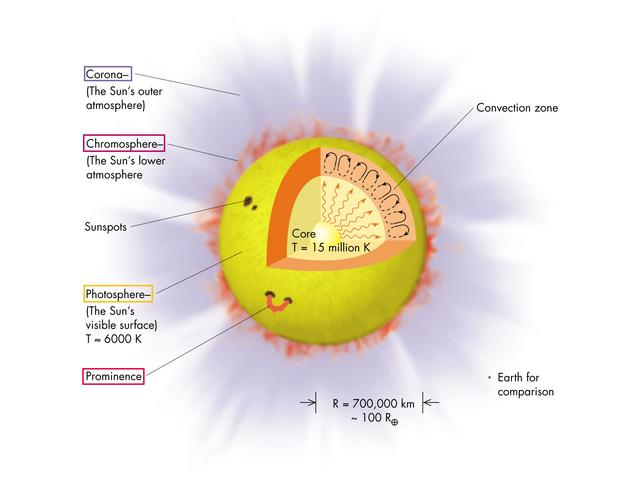
\includegraphics[trim = 0cm 0.5cm 0cm 0cm, width=1.0\textwidth]{images/solar_atmosphere}
\caption{The internal structure of the Sun, including the core, radiative zone, and convective zone.  Also shown is the structure of the its atmosphere, including the photosphere, chromosphere, and corona. The layers of the solar atmosphere are usually demarcated by temperature changes as height above the solar surface increases. The temperature ranges from $\sim$6000\,K in the photosphere to above 1\,MK in the corona.}
\label{fig:solar_atmosphere} 
\end{center}
\end{figure}



\subsection{Solar Dynamo and Magnetic Field}\label{sec:11}

\begin{itemize}
\item Cellular pattern in photosphere is very different to the convective structure in deeper layers.
\end{itemize}


\begin{figure}[!h]
\begin{center}
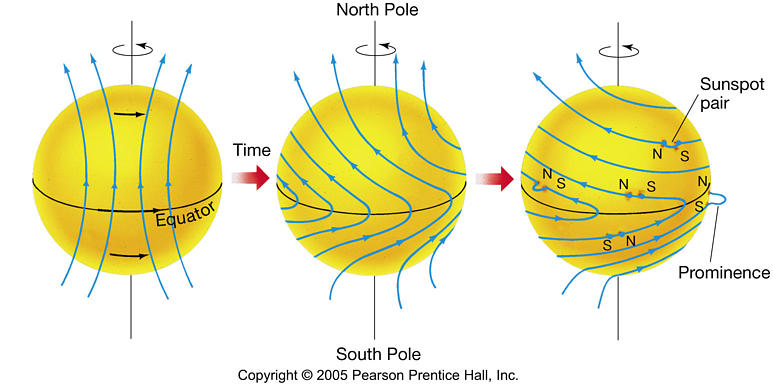
\includegraphics[]{images/Babcock}
\caption{Differential rotation and flux freezing result in the poloidal dipolar magnetic field, generated by dynamo action, to be dragged around in a toroidal direction, an action known as the omega effect. Buoyancy of the field lines results in them rising and twisting, known as the alpha effect, eventually surfacing to become bipolar fields that extend far into the corona.}
\label{fig:Babcock} 
\end{center}
\end{figure}

It is widely believed that the Sun's magnetic field is created by a dynamo action in a region between the radiative zone and the convection zone, known as the tachocline. Solar dynamo theory attempts to explain the observed 11 year magnetic activity cycle, where the the Sun's magnetic field starts as a poloidal dipolar structure and evolves to having a strong toroidal component, after which it returns to a poloidal field again. During these 11 years the Sun starts at minimum activity, reaches a maximum and returns to minimum again.

\citet{babcock1961} first explained this process by a mechanism involving differential rotation of the solar surface and interior. The equatorial rotation rate is faster than the rotation rate at higher latitudes. Because the magnetic field is frozen into the plasma, any flows in the solar interior will tend to drag the magnetic field along. By this effect, differential rotation tends to drag the field and wrap it around the Sun in a toroidal direction, this is known as the omega effect, see Figure~\ref{fig:Babcock}.

As the toroidal field builds up in the solar interior, sections of field lines build up in magnetic pressure resulting in a buoyancy of the field. The field slowly rises through the convection zone and eventually surfaces as a bipolar region that extends into the solar atmosphere. The presence of bipolar fields in the solar atmosphere and their slow build up over time to complex magnetic structures, known as active regions, ultimately leads to a variety of eruptive phenomena.



\subsection{Solar Atmosphere}\label{sec:12}

\subsubsection{Photosphere}\label{sec:121}

\begin{itemize}
\item Appearance, Granules, Sunspots.
\item Black Body Curve. Franhofer lines, H-alpha line, CaII H \& K, H$^{-}$ alines, Sodium D lines. 
\item Temperature, Density, Opacity.
\item Magnetic field strength
\end{itemize}

The most spectacular and energetic phenomena in our solar system have their origins in the solar atmosphere. This ever-changing and dynamic environment is a hotbed of activity giving rise to coronal mass ejections (CMEs), solar flares, and a host of plasma processes resulting in emission across the entire electromagnetic spectrum. To make sense of the phenomena we observe we must first have a basic understanding of solar atmospheric structure and the environment these processes take place in. Figure~\ref{fig:solar_atmosphere} is an illustration of the different layers of the solar interior, the solar surface and atmosphere. The visible surface of the Sun is known as the photosphere. It is demarcated where optical depth becomes unity for a wavelength of 5000\,\AA\ or $\tau_{5000}=1$. At such visible wavelengths, the electromagnetic spectrum is well represented by a blackbody of temperature T$\sim$6000\,K. .

\begin{itemize}
\item Eddington Barbier, $\tau=\mu$, limb darkening.
\item Effective temperature, $\tau=2/3$, $T=5800$\,K
\end{itemize}

During periods of increased activity there may also be the presence of sunspots in the photosphere. These are dark features on the solar surface, see Figure~\ref{fig:solar_atmosphere}, and are an indicator of concentrations of magnetic fields that are stronger than elsewhere in the quiet sun, as described above. 

Photospheric abundances have been measured using emission line diagnostics were it is found that helium is the most abundant at 10.89\footnote{Abundances quoted relative to hydrogen on a logarithmic scale, $12.0+log_{10}(A/A_H)$}, with the next most abundant elements being Carbon (8.58), Nitrogen (8.02), and Oxygen (8.8). All other elements have abundances that are 4 orders of magnitude or more less than hydrogen i.e., logarithmic abundances $\lesssim7$ \citep{phillips2008}.

\subsubsection{Chromosphere}\label{sec:122}

\begin{itemize}
\item Appearance, Supergranular Network, Bright Points, Spicules, Filaments, Plage etc.
\item Emission lines, H-alpha, CaII H \& K. 
\item Temperature, Density, Opacity.
\item Magnetic field strength.
\end{itemize}

At $\sim$500\,km above the $\tau_{5000}=1$ surface the temperature drops to a minimum of $\sim$4400\,K. Beyond this minimum the temperature begins to rise again, demarcating the beginning of the chromosphere. This layer of the atmosphere is generally accepted to extend to a height at which temperatures reach 20,000\,K, however temperatures as high as $\sim1\times10^5$\,K are sometimes attributed to chromospheric heights, hence it is observable at ultraviolet (UV) wavelengths as well as visible. 

\subsubsection{Corona}\label{sec:123}

\begin{itemize}
\item Appearance UV: Active regions, Coronal Loops, Holes.
\item Emission lines, Mg, Ca, Fe, C, O etc.
\item Appearance White-Light: Streamers, K, F, E corona
\item Appearance Radio: thermal bremsstrahlung, free-free emissivity/opacity.
\item Temperature, Density, Opacity, 'coronal heating problem'.
\end{itemize}


At a height of approximately 2,000\,km the temperature begins to rise sharply while the number density of neutral hydrogen and electrons fall by several orders of magnitude. This rapid increase in temperature in such a short spatial extent ($<$100\,km) is known as the transition region. It has a temperature on the order of $10^5$\,K and separates the relatively low temperature chromosphere and the high temperatures of $>1$\,MK in the corona. The reason for this rapid increase in temperature is still a hotly debated subject and a coronal heating mechanism remains largely unknown, this is known as the  \textquoteleft coronal heating problem'.


Element abundances in the corona show there is a similar composition to the photospheric abundances, with He, C, N, and O having the same ratios relative to H in the corona as that in the photosphere. The only difference is an enhancement in the abundance of low First Ionization Potential ($<10$\,eV) elements in the corona relative to the photosphere. For example, elements such as Na, Mg, Al, Si, Ca, Ni, and Fe can be up to three times more abundant in the corona \citep{feldman2003}. The reason for the enhancement of low FIP elements in the corona is still unknown, however several models have suggested ion-neutral separation in the chromosphere by diffusion across magnetic fields, followed by transport of these ions into the corona may be viable mechanism \citep{geiss1985}. 


\subsection{Solar Wind}\label{sec:13}

\begin{itemize}
\item Parker's solution
\item Parker Spiral
\item Fast solar wind, Alfv\'{e}n wave driver
\item Mass loss rates (later compare CME mass loss)
\end{itemize}



\section{Coronal Mass Ejections and Coronal Shocks}\label{sec:2}

\subsection{CMEs}\label{sec:20}

\begin{itemize}
\item Appearance, white-light Illing, Hundhausen, Vourlidas
\item Kinematics, velocity, acceleration
\item Dynamics, masses, energies, forces
\item Observations at other wavelengths, EUV, radio, SXR.
\end{itemize}

\subsection{CMEs and Shocks}\label{sec:21}

\begin{itemize}
\item Radio bursts, Type II, Type III
\item Radio imaging of shocks
\item Relationship to EUV waves, Moreton waves
\end{itemize}

\subsection{Open Questions}\label{sec:22}






	
%!TEX root = ../thesis.tex
%Adding the above line, with the name of your base .tex file (in this case "thesis.tex") will allow you to compile the whole thesis even when working inside one of the chapter tex files
\singlespacing
\chapter{Coronal Mass Ejection and Plasma Shock Theory} 
\label{chap:2}
\doublespacing
This chapter introduces the theory used to study coronal mass ejections and coronal shocks. Since the corona is a plasma, the theoretical framework under which all coronal phenomena are treated is in plasma physics and a fluid description of plasmas known as magnetohydrodynamics (MHD). Coronal mass ejections are a large scale phenomena and can therefore be treated using MHD. While plasma shocks on the large scale may also be treated in an MHD continuum framework, it is necessary to consider individual particle motions when describing particle acceleration and radio emission in shocks, requiring a departure from MHD and the use of distribution functions, the Boltzmann equation, and individual particle kinematics. Therefore, both the MHD equations and the Boltzmann equation are presented in this chapter, followed by an application of this theory to CMEs and plasma shocks.

\singlespacing
\section{Plasma Physics and  \\ Magnetohydrodynamics}\label{sec:1}
\doublespacing
\subsection{Maxwell's Equations}\label{sec:10}

Since plasmas are an electrically conducting fluid which may interact with electromagnetic fields, Maxwell's equations are an essential starting point for all plasma theory. Maxwell's equations form a closed set of four unknowns and four equations describing relationships between the electric field $\mathbf{E}$, the magnetic field $\mathbf{B}$, the current density $\mathbf{j}$, and the charge density $\rho_q$
\begin{eqnarray}
\nabla \cdot \mathbf{E} &=& \frac{\rho_q}{\epsilon_0} \\
\nabla \cdot \mathbf{B} &=& 0 \\
\curl{\mathbf{E}} &=& - \frac{d\mathbf{B}}{dt} \\
\curl{\mathbf{B}} &=& \mu_0 \mathbf{j} + \frac{1}{c^2}\frac{d\mathbf{E}}{dt} 
\end{eqnarray}
$\mu_0$ and $\epsilon_0$ are the magnetic permeability and electric permittivity of free space, respectively, and all bold face quantities represent vector variables. At velocities typically found in a plasma equation (2.4), Amp\'{e}re's law, reduces to
\begin{equation}
\curl{\mathbf{B}} = \mu_0 \mathbf{j}
\end{equation}
where the displacement current is no longer included. Maxwell's equations describe electromagnetic behaviour and they constitute an important part of the fluid description of plasmas. Before we define this fluid description a brief discussion of plasma kinetic theory, from which the fluid theory is derived, is provided here.

\subsection{Plasma Kinetic Theory}\label{sec:11}

The general approach to the majority of plasma phenomenon is in a collective description using particle distribution functions and the use of differential equations to describe the evolution of these distribution functions. This is known as plasma kinetic theory, and the distribution functions can be of the form of the Maxwell-Boltzmann velocity distribution, while the differential equation used to describe its evolution is the Boltzmann equation. Many non-equilibrium or unstable states of a plasma, such as those that produce radio bursts described in sections~\ref{sec:wave_particle}--\ref{sec:three_wave} require a kinetic theory description of plasma. A brief overview of kinetic theory is therefore given here before describing specifically its application to plasma emission and radio bursts.

As with a neutral gas, the particle distribution function $f(\mathbf{r}, \mathbf{v}, t)d\mathbf{v}d\mathbf{r}$ described the number of particles having positions between $\mathbf{r}$ and $\mathbf{r}+d\mathbf{r}$ and velocities between $\mathbf{v}$ and $\mathbf{v}+d\mathbf{v}$, at time $t$. This distribution function can be used derive a number of useful physical properties of the plasma, such as the particle number density at position $\mathbf{r}$ and time $t$ 
\begin{equation}
n(\mathbf{r},t) = \int f(\mathbf{r}, \mathbf{v},t) d \mathbf{v}
\label{eqn:num_density}
\end{equation}
as well as the bulk velocity particle velocity, given by
\begin{equation}
 \mathbf{v}(\mathbf{r},t) = \frac{1}{n(\mathbf{r},t)}\int  \mathbf{v} f(\mathbf{r}, \mathbf{v},t) d \mathbf{v}
\label{eqn:bulk_flow}
\end{equation}
The evolution of this distribution function in time and space is described by the Boltzmann equation, given by
\begin{equation}
\frac{\partial f(\mathbf{r}, \mathbf{v},t)}{\partial t}  +     ( \mathbf{v}\cdot\nabla_r)f(\mathbf{r}, \mathbf{v},t)    + (\mathbf{a}\cdot\nabla_v)f(\mathbf{r}, \mathbf{v},t) = \bigg(\frac{\partial f(\mathbf{r}, \mathbf{v},t)}{\partial t}\bigg)_{coll}
\label{eqn:boltzmann}
\end{equation}
This equation describes the changes in occupation number of particles at positions ($\mathbf{r}, \mathbf{v}$, t) in phase space due to a configuration space flux $\mathbf{v}\cdot\nabla_rf$, a velocity space flux $ \mathbf{a}\cdot\nabla_vf$, as well as collisions experienced by the particles (last term in the right). Equation~\ref{eqn:boltzmann} is the fundamental basis of all plasma and neutral gas kinetic theory and provides a very powerful tool for describing the time and space evolution of equilibrium and, more importantly, non-equilibrium distributions of particles. It is the most general description of the behavior of an ensemble of particles, and all other macroscopic fluid dynamical equations may be derived from it.

Assuming  the plasma to be collisionless and stating the accelerations in the plasma in terms of the electric field $\mathbf{E}$ and magnetic field $\mathbf{B}$, Equation~\ref{eqn:boltzmann} may be reduced to the Vlasov equation for a plasma interacting with electromagnetic fields.
\begin{equation}
\frac{\partial f}{\partial t}  +(\mathbf{v}\cdot\nabla_r)f + (\frac{q}{m}[\mathbf{E} + \mathbf{v}\times \mathbf{B}]\cdot\nabla_v)f = 0
\end{equation}
where $q$ is Coulomb charge, $m$ is particle mass, and $f(\mathbf{r}, \mathbf{v},t)$ is reduced to $f$ for simplicity of notation. This form of the Vlasov equation is used in the formulation of wave-particle interactions, and wave growth in plasmas, that ultimately lead to plasma emission in solar radio bursts, this will be described in further detail sections~\ref{sec:wave_particle}--\ref{sec:three_wave}.

In equations \ref{eqn:num_density} and \ref{eqn:bulk_flow}, the number density and bulk velocity of the plasma were obtained by taking appropriate weighted integrals of the distribution function. This is done to obtain information on the macroscopic properties of the plasma when the specific details of the particle distribution are not needed. A behaviour of the plasma on a macroscopic or fluid scale may be obtained by taking the appropriate integrals of the the Boltzmann equation in a procedure known as `taking the moments of the Boltzmann equation'. The moments of a function are given by 
\begin{equation}
\mu_n = \int x^n f(x) dx
\end{equation}
where the $n$ describe the moments e.g., $n=0$ is the {\it zeroth moment},  $n=1$ is the {\it first moment} etc. Taking the moments of the Boltzmann equation lead to a set of fluid conservation equations that describe the dynamics of a plasma on a continuum scale (no individual particle motion available). The moments are as follows
\begin{eqnarray*}
\int [\mathrm{Boltzmann~ eq.}]\times v^0 dv &\rightarrow& \mathrm{conservation~of~mass} \\
\int [\mathrm{Boltzmann~eq.}]\times v^1 dv &\rightarrow& \mathrm{conservation~of~momentum} \\
\int [\mathrm{Boltzmann~eq.}]\times \frac{v^2}{m} dv &\rightarrow& \mathrm{conservation~of~energy}
\end{eqnarray*}
In their most fundamental form, these conservation equations are used in what is known as a multi-fluid description of the plasma, where the dynamics and conservations of the various properties are treated seperately for each particle species e.g., electrons and protons will have different conservation equations and described separately as an \textquoteleft electron fluid' and \textquoteleft proton fluid'. However, combining these separate fluids into one \textquoteleft single fluid' framework constitutes a description of plasmas known as magnetohydrodynamics\footnote{The moments of the distribution function and the reduction of multi-fluid to single fluid conservation equations involve lengthy derivations that are not provided here but can be found in many texts \citep{goossens2003, inan2011}.}.

\subsection{Magnetohydrodynamics}\label{sec:12}
The conservation principles  derived from moments of the Boltzmann equation are firstly the mass conservation equation
\begin{equation}
\frac{D\rho}{Dt} = -\rho\nabla\cdot \mathbf{v}
\end{equation}
where $\rho$ is mass density, $\mathbf{v}$ is bulk flow velocity, $t$ is time, and $D$ represents a Lagrangian derivative ($D/Dt = \partial /\partial t + v\cdot \nabla$). This expression simply states that the rate of change of particles into or out of a volume is controlled by the fluid flow into and out of the volume. It has units of kg\,m$^{-3}$\,s$^{-1}$.

Secondly, the momentum conservation equation is
\begin{equation}
\rho\frac{D\mathbf{v}}{Dt}=-\nabla p + \mathbf{j}\times \mathbf{B} + \mathbf{f} +\nabla \cdot \mathbf{S}
\label{eqn:mhd_momentum}
\end{equation}
where $p$ is thermal pressure, $\mathbf{j}$ is the current density, $\mathbf{B}$ is the magnetic field, $\mathbf{f}$ are all body forces e.g., gravity, and $\mathbf{S}$ is a stress tensor. This equation shows that the change in momentum of a fluid may be due to a pressure gradient, the \textquoteleft j cross B' or Lorentz force, gravity, and any stresses in the plasma e.g., kinematic viscosity $\nu$. Note that with $\nabla \cdot \mathbf{S}=\rho\nu\nabla^2\mathbf{v} $, and setting gravity and the Lorentz term to zero gives the Navier-Stokes equation of motion of a viscous fluid. Note that all terms in this equation have the form of a body force (force per unit volume), and integration over volume would render this equation an explicit version of Newton's second law ($m\mathbf{a}=\mathbf{F}$).

The third conservation equation is the energy conservation equation
\begin{equation}
\rho\frac{De}{Dt} + p\nabla\cdot \mathbf{v}=\nabla\cdot(\kappa\cdot\nabla T) +  \eta_e\mathbf{j}^2 + Q_{\nu} - Q_r
\end{equation}
where 
\begin{equation}
e = \frac{p}{(\gamma-1)\rho}
\end{equation}
is the internal energy per unit mass, $\gamma$ is the ratio of specific heats, $\kappa$ is the thermal conductivity, $T$ is the temperature, $\eta_e$ is electrical resistivity, $Q_{\nu}$ is heating by viscous dissipation, and $Q_r$ is a radiative term. This equation demonstrates that any changes in the fluid internal energy are due to divergence in the flow field, conduction, ohmic and vicious dissipation, and radiative losses.

The fluid momentum equations can be used to formulate Ohm's law for a plasma which describes the behaviour of current in terms of electric and magnetic fields and the fluid flow velocity
\begin{equation}
\mathbf{j} = \sigma(\mathbf{E} + \mathbf{v}\times \mathbf{B})
\end{equation}
This is a reduced version of the generalised Ohm's law and does not contains terms for the Hall effect, ambipolar diffusion, and electron intertia. The set of equations (2.11 - 2.15), combined with an equation of state 
\begin{equation}
p = nk_BT
\end{equation}
results in a fully closed set of variables and equations, which can be solved for any fluid or electromagnetic property. In order to further simplify these set of equations the electric field $\mathbf{E}$ and current $\mathbf{j}$ are often eliminated by using Faraday's law in combinations with Amp\'{e}re's and Ohm's law to produce the induction equation
\begin{equation}
\frac{\partial \mathbf{B}}{\partial t} = \nabla \times(\mathbf{v}\times \mathbf{B}) + \eta\nabla^2 \mathbf{B}
\end{equation}
which describes the evolution of the magnetic field in terms of the plasma flow and the magnetic diffusivity $\eta = \eta_e/\mu_0$.  The mass, momentum, internal energy equation, the induction equation, and the solinoidal constraint then define  a fully closed system of resistive MHD equations in terms of the variables ($\mathbf{B}, \mathbf{v}, p, \rho$)
\begin{eqnarray}
\frac{D\rho}{Dt} = -\rho\nabla\cdot \mathbf{v} \\
\rho\frac{D\mathbf{v}}{Dt}=-\nabla p + \frac{1}{\mu_0}(\nabla \times \mathbf{B})\times \mathbf{B} + \mathbf{f} \\
\frac{D\rho}{Dt} = -\gamma p\nabla\cdot \mathbf{v} +(\gamma -1)\frac{\eta}{\mu_0^2} (\nabla \times \mathbf{B})^2 \\
\frac{\partial \mathbf{B}}{\partial t} = \nabla \times(\mathbf{v}\times \mathbf{B}) + \eta\nabla^2 \mathbf{B} \\
\nabla\cdot \mathbf{B} = 0
\end{eqnarray}
It is also assumed here that the fluid is inviscid and not subject to any conductive or radiative energy losses or gains. Under this reduced set of equations, the ideal MHD equations are simply produced by setting $\eta = 0$ e.g., zero resistivity, which would eliminate the second terms on the right in equations 2.20 and 2.10. Under such an assumption the ideal induction equation
\begin{equation}
\frac{\partial \mathbf{B}}{\partial t} = \nabla \times(\mathbf{v}\times \mathbf{B})
\end{equation}
may be used to show the \textquoteleft frozen flux' condition. This shows that when $\eta = 0$ the field is advected with the plasma or the field is \textquoteleft frozen-in' into the plasma and follows the flow velocity i.e., there is no `slipping' of the magnetic field with respect to the fluid flow.  On the other hand, a finite $\eta$ leads to a variety of important diffusive effects for the magnetic field. The most important of these diffusive processes is magnetic reconnection, which plays an extremely important role in solar flares and CMEs.



%-----------------------------------------------------------%
%		   Magnetic Reconnection	                 % 
%-----------------------------------------------------------%
\subsection{Magnetic Reconnection}\label{sec:13}

If the dissipation of concentrations of magnetic flux in the solar corona are due to diffusion processes only, a timescale for this diffusion process may be estimated from the magnetic induction equation. Assuming the diffusion term dominates over advection term
\begin{equation}
\frac{\partial B}{\partial t} = \eta\nabla^2\mathbf{B}
\label{egn:diff}
\end{equation}
As an order of magnitiude estimate for the derivatives we replace $\partial/\partial t \rightarrow 1/\tau_D$ and $\nabla^2 \rightarrow 1/L^2$. Equation~\ref{egn:diff} then gives
\begin{equation}
\tau_D = \frac{L^2}{\eta}
\label{eqn:diff_time}
\end{equation}
The typical length scales for a coronal active region are $10^7$\,m, and assuming a Spitzer magnetic diffusivity $\eta = 10^9T^{-3/2} = 1$\,m$^2$\,s$^{-1}$ \citep{spitzer1962}, equation~\ref{eqn:diff_time} gives a diffusive timescale of 3.1 million years.
Given that active regions evolve quasi-statically over weeks and evolve dynamically over timescales of seconds and minutes during a flares and CMEs, there must be an evolution process other than a large scale diffusion in the solar atmosphere. Equation~\ref{eqn:diff_time} indicates that there may be two different ways in which the evolution of magnetic fields may occur over a much shorter times scale: either the typical length scale $L$ is much shorter, or magnetic diffusivity $\eta$ is much larger.

Magnetic reconnection is the dynamical process that describes the short timescale evolution of magnetic fields in the corona (and other astrophysical and laboratory systems). It involves a change in magnetic topology that converts magnetic energy in kinetic and thermal energy of the bulk plasma and accelerates particles to high speeds. Magnetic reconnection typically occurs in a boundary between two oppositely directed magnetic field regions. At the very center of the boundary layer the magnetic field must go to zero to account for a continuous change from positive to negative magnetic field. The total pressure balance in the boundary layer and on either side is \citep{asch2004}
\begin{equation}
B_1 + p_1 = p_{dr} = B_2 + p_2
\end{equation}
where $p_{1,2}$ and $B_{1,2}$ represent thermal and magnetic pressure on either side of the diffusion region, respectively, and $p_{dr}$ is the pressure inside the diffusion region (no magnetic pressure).


\begin{figure}[!t]
\begin{center}
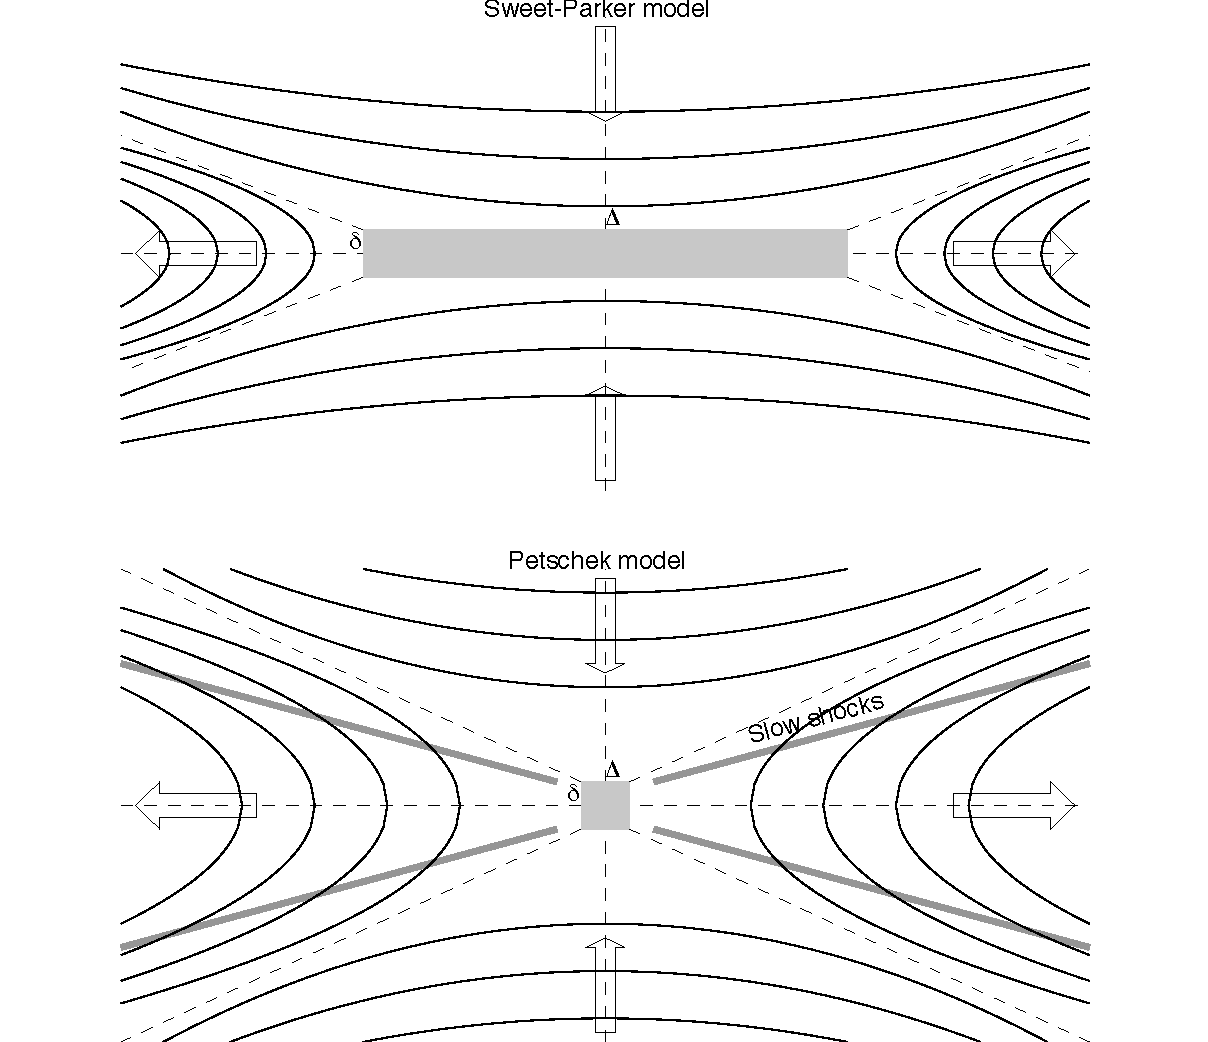
\includegraphics[scale=0.7]{reconnection.pdf}
\caption[Sweet-Parker and Petscheck reconnection models]{The reconnection models of Swee-Parker (top) and Petscheck (bottom). The Sweet-Parker mechanism employs a long and thin ($\Delta>>\delta$) current sheet as the diffusion region. It produces reconnection rates that are much too slow to describe flare and CME energy dissipations rates. Petscheck proposed a similar model but with a diffusion region that is much smaller, with $\Delta\approx\delta$, resulting in reconnection rates that are consistent with flare and CME timescales. The dissipation of energy in this model is partly controlled by the presence of two slow-mode shocks which separate the sub-Alfv\'{e}nic inflow region and the super-Alfv\'{e}nic outflow region \citep{asch2004}.}
\label{fig:recconection}
\end{center}
\end{figure}
The existence of inflows into the diffusion region at right angles to the magnetic field creates an electric field in this layer that is perpendicular to the inflow plane. This creates a current in the diffusion region, hence this ayer is often called a `current sheet'. The diffusion of magnetic fields occurs within this current sheet. Sweet and Parker were the first devise a mechanism by which magnetic reconnection occurs in such a current sheet \cite{sweet1958, parker1963}. 
%Although no complete analytical theory exists for the process, the MHD conservation equations may be applied to derive the reconnection rate. The application of resistive MHD only applies within the thin current sheet, while ideal MHD applies everywhere else.

The Sweet-Parker were the first to devise a model whereby the diffusive time scale of the field (equation~\ref{eqn:diff_time}) could be made much faster by considering a diffusion region much smaller than the size scales of active regions. The model consists of a current sheet (diffusion region) that is much longer than it is wide i.e., in the top panel of Figure~\ref{fig:recconection} $\Delta>>\delta$, where $\Delta$ is current sheet half-length and $\delta$ is current sheet half-thickness. Conservation of mass implies that the rate at which mass enters the sheet must equal the rate that mass exits the sheet
\begin{equation}
\rho \Delta v_{in} = \rho \delta v_{out}
\label{eqn:in_out}
\end{equation}
where $v_{in}$ and $v_{out}$ are the inflow and outflow speeds respectively. Using equations~\ref{eqn:diff_time} and \ref{eqn:in_out} the inflow speed may be written as
\begin{equation}
v_{in}^2 = \frac{\eta v_{out}}{L}
\end{equation}
The reconnection rate depends on in the ratio of the inflow speed $v_{in}$ to the outflow speed $v_{out}$ in the form of the Mach number
\begin{equation}
M = \frac{v_{in}}{v_{out}} = \frac{1}{\sqrt{S}}
\end{equation}
where $S=v_AL/\eta$ is the Lundquist number (equivalent to the magnetic Reynold's number at the Alfv\'{e}n speed). The rate of reconnection depends on the length scale and magnetic diffusivity in the current sheet. Despite the fact that the Sweet-Parker mechanism provides a rate of magnetic energy dissipation that is faster than the global process, it is much too slow to explain the process of magnetic energy release in solar flares. For example for typical Lundquist numbers of $10^{12}$, the Sweet-Parker model produces a reconnection rate of $10^{-6}$ of the Alfv\'{e}n speed.

To over come the problem, Petscheck proposed a model with a much smaller diffusion region where $L\approx\delta$ \citep{petschek1964} . With this smaller diffusion region, the boundary between inflow and outflow regions are separated by slow mode magnetoacoustic shocks. Alongside the diffusion region, these shocks also help to dissipate some of the inflowing kinetic energy into thermal energy. Again, no analytical solution to the model exists but Petscheck found that when the diffusion regions is allowed to be small, the reconnection rate is given as
\begin{equation}
M \approx \frac{\pi}{8\,\mathrm{ln}(S)}
\end{equation}
This gives a much faster reconnection rate of 0.01 of the Alfv\'{e}n speed (hence it is known as fast reconnection), which is comparable to solar flares. When Petscheck presented the model it was thought to be a complete description of 2D magnetic reconnection, however other solutions would soon be discovered, with the Petscheck model being just one of a family of possible 2D reconnection mechanisms. These mechanisms describe steady, uniform, 2D reconnection, the rate of which may be summarised as \citep{priest1986}
\begin{equation}
\bigg(\frac{M_e}{M_e}\bigg)^2 \approx \frac{4M_e(1-b)}{\pi}\bigg[ 0.834 -\mathrm{ln \, tan}\bigg( \frac {4S\sqrt{M_eM_i}} {\pi}  \bigg)^{-1}\bigg]
\end{equation}
This contains the Sweet-Parker, the Petscheck ($b=0$) and Sonnerup \citep{sonnerup1970}($b=1$) reconnection rates.

%While these solutions show that 2D reconnection may be explained well by MHD, describing 3D reconnection remains big theoretical and computational challenge, and remains at the forefront of reconnection theory research. Both 
2D reconnection, an the more complicated 3D models, play a role in many theoretical models describing the eruption of coronal mass ejections and flares. Although some CME models have no need for reconnection to occur, there is a growing consensus that it is an integral part of the solar eruptive process.

%-----------------------------------------------------------%
%		       CME Theory			        % 
%-----------------------------------------------------------%

\section{Coronal Mass Ejections}\label{sec:2}

Magnetohydrodynamic models of eruptive coronal mass ejections use either ideal or resistive MHD (without and with reconnection, respectively) to bring about a loss of equilibrium of some complex magnetic structure in the corona. The magnetic structure usually takes the form of a flux rope, a helical or twisted magnetic structure embedded in the coronal magnetic field. The main goal of every model is to induce a loss of equilibrium of the structure, but the mechanism by which this is done varies greatly amongst the models. {\it Storage models} assume a slow build up of magnetic stress in a non-potential field that may store free energy over long time scales before some loss of equilibrium occurs and the stored magnetic energy is rapidly converted to mechanical energy and the expulsion of a magnetic structure \citep{wolfson1998, forbes1995, antiochos1999}. {\it Dynamo models} involve a rapid generation of magnetic flux by either stressing of the field or flux-injection into the system. As the name suggests, these models usually consider the interplay between current and magnetic field in the system that may bring about a Lorentz force which provides an expulsion of the flux rope from the low corona \citep{chen1989, krall2001, schrijver2008, fan2005}. Finally there are the {\it thermal blast models}, which produce an expulsion of the CME into interplanetary space by an enhanced pressure gradient due to the rapid heating of a flare i.e., an explosive ejection of plasma from the corona.  This model is somewhat out-dated now since CMEs are no longer thought to be the result of flares, with some CMEs preceding flare onset and some occurring without any flare \citep{gosling1993}.

The main goal of every model is to induce a loss of equilibrium of the structure, but the mechanism by which this is done varies greatly amongst the models e.g., there is still some debate on whether the flux rope is formed as a result of eruption or it is a pre-existing structure. The need for reconnection is also a source of contention, with some models inducing eruption using only ideal MHD and other models employing resistive MHD \citep{chen2011}. The most prominent of these models are discussed here.

\subsection{Catastrophe Model}\label{sec:20}
\begin{figure}[!t]
\begin{center}
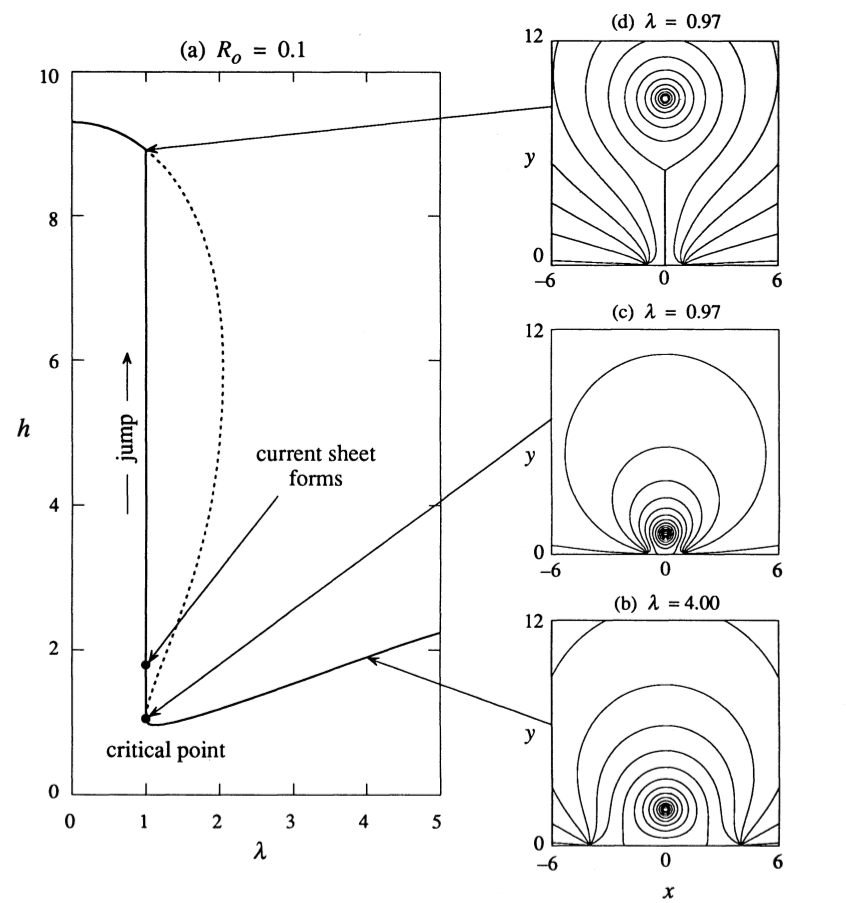
\includegraphics[scale=0.4, trim=1cm 1cm 0cm 1.5cm]{images/catastrophe}
\caption[The catastrophe CME model]{The catastrophe model of \citep{forbes1995}. The model consists of a 2D pre-existing flux rope with foot points rooted in the photosphere. The fluxrope is driven toward instability by motions of the photospheric footpoints, in this case the distance between the footpoints $\lambda$ decreases slowly (timescales much longer than the Alfv\'{e}n crossing time $\tau=L/v_A$). As the foot points converge the fluxrope initially contracts indicated by a decreasing height in panel (a). Eventually this convergence brings the system to critical point where magnetic pressure outwards dominates inward magnetic tension. The system rises, reaches a new equilibrium position, and forms a current sheet. The evolution of the system after it reaches this new equilibrium largely depends on whether or not magnetic reconnection occurs in the sheet. the rate of reconnection may also bring about different evolutions in kinematics \citep{priest2000}.}
\label{fig:catastrophe}
\end{center}
\end{figure}

The catastrophe model assumes a flux-rope is formed in the corona prior to eruption and considers the balance between magnetic tension holding the flux rope in position, and magnetic pressure (from compression of field lines under the rope) that supply an outward directed force \citep{forbes1991, lin2000, priest2000}. A loss of equilibrium is brought about by photospheric motions, either convergence or shearing of the foot points, which are well-known precursors to eruptive activity in the corona \citep{rust1972}. the reduction of the distances between the foot points, $2\lambda$, decreases and this initially 
causes an increase in the magnetic tension which makes the rope contract and reduce its height Fig.~\ref{fig:catastrophe}. However, continued contraction results in a magnetic compression that  dominates tension, resulting in a flux rope rise. As the rope rises it forms a current sheet behind it, and its evolution after this point depends on whether or not reconnection occurs in the current sheet. If no reconnection is present then the flux rope simply rises and finds a new equilibrium position at a greater height, in this case the net release of magnetic energy is less than 1\% of the energy stored in the pre-field configuration \citep{forbes1991}. If reconnection occurs, then the eruption proceeds uninhibited and up to 95\% of the stored magnetic energy is released \citep{forbes1995}.

\citet{forbes1995} provided expressions for the development of current in the flux rope with respect to height which was used to estimate the free magnetic energy in the system. By assuming a rapid reconnection rate, and that all of this free energy was converted to the rope's kinetic energy they were able to derive velocity-time kinematics, and under the constraint of the flux rope radius $a\rightarrow 0$ an analytical expression for the rope velocity may be derived as \citep{priest2000}
\begin{equation}
v\approx \sqrt{  \frac{8}{\pi}  }v_{A0}\bigg[\mathrm{ln}\bigg( \frac{h}{\lambda_0}\bigg) + \frac{\pi}{2}  - 2\mathrm{tan}^{-1} \bigg( \frac{h}{\lambda_0}\bigg)\bigg] + v_0
\end{equation}
where $h$ is the fluxrope height, $2\lambda_0$ is the foot point separation at $\lambda=h$, $v_0$ is an initial perturbation velocity (1\% of the Alfv\'{e}n speed), and $v_{A0}$ is the Alfv\'{e}n speed where $\lambda=h$. Magnetic power output in the early phase of eruption is given by
\begin{equation}
\frac{dW}{dt} \approx -\frac{2A_0^2}{\pi\mu}\bigg( \frac{h}{\lambda_0} -1\bigg)^2\frac{v}{\lambda_0}
\end{equation}
where $h\sim t + t^{5/2}$ and $v\sim t^{3/2}$ i.e., the initial power output grows with time. In the later phases of propagation the power output decays with time as
\begin{equation}
\frac{dW}{dt} \approx \frac{4A_0^2}{\pi \mu t}
\end{equation}
so the growth in power output occurs approximately 100 times quicker than the decay in power output.

A later study by \citet{priest2000} analysed how reconnection in the underlying current sheet may influence the eruption of the flux rope. The kinematics of the rope after equilibrium is lost depend on the rate of reconnection in the sheet, parameterised by the Alfv\'{e}n Mach number of the inflow into the reconnection site. If $M_A=0$ then the fluxrope does not escape but oscillates around an equilbrium height like a yo-yo. If $0<M_A<0.005$, escape is possible but the rope may show a number of oscillations in height before escape, this behaviour has never been directly observed so reconnection must occur at a rate $M_A>0.005$ to produce eruption.  For $0.005<M_A<0.041$ to rope escapes but undergoes a period of deceleration between 20 and 100 Alfv\'{e}n crossing times, while for $M_A > 0.041$ no deceleration occurs and the fluxrope escapes and approaches an asymptotic velocity.

The catastrophe model provides a successful way of evolving a flux system to the point of catastrophic loss of equilibrium and consequent eruption. However, a major limitation is that it is a 2D model and does not take into account that the ends of the flux rope will be anchored in the photosphere. This would produce a curvature in the rope that would increase its tension and hence change the dynamics, but it is unlikely that it would prevent eruption \citep{steele1989}




\subsection{Magnetic Breakout Model}\label{sec:21}

The magnetic breakout model was first proposed by \citep{antiochos1999} and involves a quadrupolar (or more complex) magnetic flux system. A core magnetic field is flanked by two side-lobe fields, which collectively lie underneath an over-arching field that stabilizes the whole system. The overarching field and core field are almost anti-parallel, creating a magnetic null point between the two Figure~\ref{fig:breakout_model}. Non potentiality is injected into the core by twisting/shearing of the foot points or by flux emergence. This non-potentiality causes the core field to grow and encounter the overarching field, distorting the null point into a current sheet and eventually allowing reconnection to occur. The reconnection removes field lines from the overarching field and adds it to the side-lobe systems, allowing further growth of the core field. The growth of the core field in turn drives further breakout reconnection resulting in a positive feedback required for explosive expulsion of the core. Finally, as the core is accelerated a current sheet forms in its wake, eventually leading to a separation of the core flux from the solar surface that forms a plasmoid structure typical of a three part CME \citep{lynch2004}; an important aspect of this is that flux rope formation happens as a consequence of eruption i.e., it is not pre-existing. The magnetic breakout model was used to circumvent the Aly-Sturrock limit \citep{aly1991, sturrock1991} i.e., it allowed a flux system to erupt, without having to open the constraining field lines to infinity.
\begin{figure}[!t]
\begin{center}
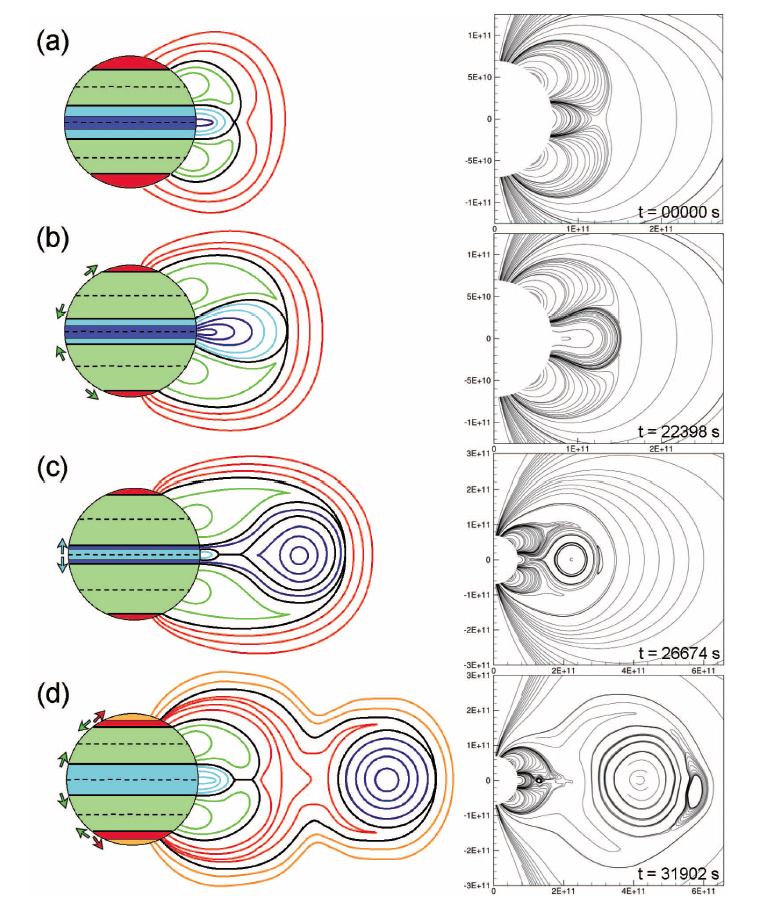
\includegraphics[scale=0.45, trim=0cm 0cm 0cm 1cm]{images/lynch_breakout}
\caption[The breakout CME model]{The breakout model, consisting of a quadrupolar flux system in which the central flux (blue) is flanked by to side lobe flux systems (green), with the entire system kept in stability by the tension of the overlying red field. Shearing and/or twisting on the underlying flux causes it to grow slowly. Eventually a current sheet forms at the magnetic null above the central flux, causing reconnection. This reconnection transfers overlying field to the side-lobes, effectively creating a conduit for the central flux to escape as a CME \citep{lynch2008}.}
\label{fig:breakout_model}
\end{center}
\end{figure}

Kinematically, the CME/central field system should experience a slow rise (1\,km\,s$^{-1}$) for several hours due to shearing/twisting of the foot points. Once breakout reconnection has begun the CME experiences a much larger acceleration (100\,km\,s$^{-1}$). The reconnection in the current sheet in the wake of the CME is the source of energetic particles that ultimately lead to flaring (ribbons and soft x-ray loops). Therefore magnetic breakout predicts that the flaring process and SXR peak should only begin after CME acceleration (after breakout reconnection) has begun \citep{lynch2004}. However, the precedence in breakout reconnection over flaring reconnection may not always be case, with the latter sometimes driving the former \citep{macneice2004}. The above studies have mainly been through 2.5\,D simulations but a 3\,D simulation of the breakout model was given in \citep{lynch2008}. This allowed a full estimate of the conversion of magnetic energy into kinetic energy. It is found that during the flare impulsive phase 17.8\% of the free magnetic energy ($4.6\times10^{31}$\,ergs) is converted into plasma kinetic energy ($8.1\times10^{30}$\,ergs). During the gradual phase the proportion of free magnetic energy converted to kinetic energy drops to 15.4\%

There has been observational tests of the magnetic-breakout model, showing it to be a viable explanation of some flaring and CME events, the most notable of which is the Bastille Day event \citep{aulan2000}. The observational signatures of the model include the presence of a null point in the corona above a complex multipolar flux system (inferred from potential field source surface extrapolations), a radio source imaged to be above the erupting structure (implying a reconnection site), and radio bursts beginning at frequencies indicative of high altitude (again indicating energy release above the erupting structure, prior to eruption) \citep{manoh2003}. However, in some instances magnetic breakout is implied by observations of the above, but the kinematics are inconsistent with model predictions. For example the model predicts a long slow rise of the central flux system as the underlying field is increasingly sheared, after which there is a rapid acceleration once breakout reconnection is initiated. However, in the study of \citet{bong2006} the breakout reconnection occurred at the end of the CME acceleration phase, prompting a two-phase acceleration scenario.


\subsection{Toroidal Instability}\label{sec:22}

The toroidal instability model incorporates a pre-existing flux rope structure that is built from a torus of magnetic flux, some of which is buried beneath the photosphere \citep{chen1989}. The flux system is can be broken down into a combination of toroidal magnetic field, toroidal current , poloidal magnetic field and poloidal current Figure~\ref{fig:chen_model}. This flux rope system is embedded in a surrounding coronal magnetic field $\mathbf{B}_{corona}$. The stability of the system depends on the nature of the $\mathbf{J} \times \mathbf{B}$ force due to the interaction toroidal and poloidal components of both the field and current. The interaction of $\mathbf{J}$ and $\mathbf{B}$ internal to the flux rope is usually termed the Lorentz self-force or the \textquoteleft hoop' force. An instability may be induced via twisting of the fluxrope footpoints to increases the amount of poloidal flux (effectively increasing the helicity of the system). The instability arrises when the outward hoop force decreses more slowly within the ring radius than the opposing Lorentz force due to an external magnetic field. Once the instability is induced, the fluxrope begins a bulk motion as well as a growth in its semi-minor axis. Hence the motion of the system can be analysed by looking at the central axis or the minor axes (leading and trailing edges). The three axes display slightly different kinematics e.g., the leading edge has a faster velocity than the trailing edge (due to fluxrope expansion). This has proved a useful test of the model when comparing the observations of erupting fluxrope structures as seen in white-light coronagraphs. \citet{krall2001} analysed the leading and trailing edges of erupting flux rope, as well as the rope aspect ratio, and compared the observations to model expectations. Good agreement is found between the model kinematics and aspect ratio and the observed events.
\begin{figure}[!t]
\begin{center}
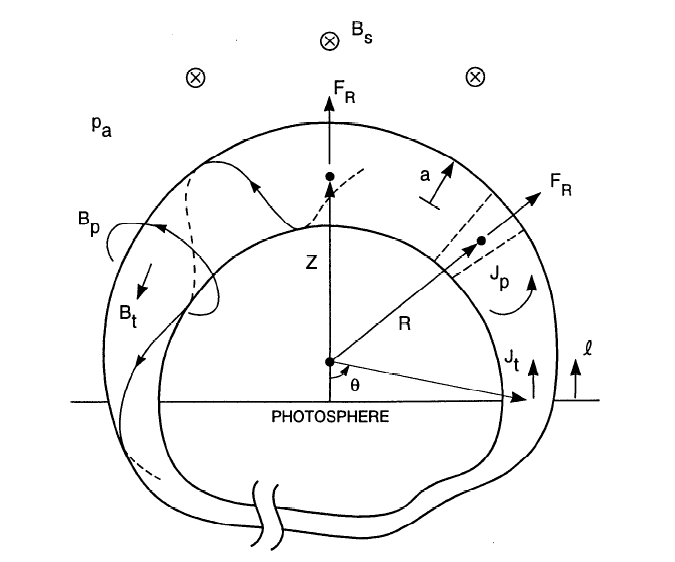
\includegraphics[scale=0.4, trim=0cm 1cm 0cm 1cm]{images/chen_model}
\caption[The toroidal instability CME model]{The flux rope model of \citet{chen1989}, used to to study the toroidal instability of a twisted flux system in the corona.}
\label{fig:chen_model}
\end{center}
\end{figure}
The equation of motion of the entire system is given by
\begin{equation}
M\frac{d^2Z}{dt^2} = \frac{I_t}{c^2R}\times\bigg[ \mathrm{ln}\bigg(\frac{8R}{a}\bigg) -1+ \frac{\xi_i}{2} + \frac{\beta_p}{2} -\frac{B^2_t}{B^2_{pa}}  -\frac{2RB_{\perp c}}{aB_{pa}} \bigg] - F_g - F_{drag}
\end{equation}
where $I_t$ is the toroidal current, $R$ is the flux rope major radius, $a$ is the rope minor radius, $\xi_i$ is internal inductance of the flux system, $B_t$ is the toroidal field, $B_{pa}$ is the poloidal field at $a$, $B_{\perp c}$ is the perpendicular component of the ambient coronal field, $F_g$ is the force due to gravity, $F_{drag}$ is the drag force, $M$ is the mass per unit length of the rope, and $Z$ is the rope axis height above the photosphere. The equation of motion shows that an increase in the toroidal current (or poloidal flux) contributes positively to the acceleration. The terms in the square brackets are each unitless and take into account the rope geometry, self-inductance and interplay between poloidal and toroidal flux. The first three terms in the square brackets are what give rise to the hoop-force. If the rope is mass loaded with a prominence, this can contribute to the rope's stability via the gravity term. The drag term only becomes an important contributor to rope dynamics later in the propagation, when the solar wind speed begins to increase i.e., at around 10$R_{\odot}$ \citep{sheeley1997}. The eruption is driven by flux-injection, which typically lasts for 4-8 hours, during which time the unstable system loses its equilibrium and begins to rise \citet{krall2001}.

It is significant the fluxrope is already established in the corona before eruption begins i.e., the rope formation is not addressed in the model and it is not a consequence of eruption. Hence magnetic reconnection is not a necessary aspect of the model and the eruption may proceed without employing resistive MHD. The model has been tested against observations and found to provide consistent result with the acceleration and jerk profiles of destabilized filaments during eruption \citep{schrijver2008}

%\subsection{Drag Models}\label{sec:23}
\section{Coronal Shocks and Plasma Emission}\label{sec:3}

\subsection{Alfv\'{e}n Speed in the Corona}
The speed at which perturbations travel in a magnetized plasma is the Alfv\'{e}n speed, given by
\begin{equation}
v_A = \frac{B_0}{\sqrt{\mu_0 \rho}}
\end{equation}
where $B_{0}$ is the unperturbed (equilibrium) magnetic field, $\mu_{0}$ is the magnetic permeability, and $\rho_{0}$ is the unperturbed mass density of the medium. This is a highly anisotropic wave driven by the restoring force of magnetic tension, with the inertia provided by the plasma mass density. Perturbations in the magnetic field, $B_{1}$, are transverse to the direction of $B_0$ and the group velocity always has a wave $\hat{k}$ vector parallel to the magnetic field direction. The quiet solar corona in the range of $1-3$\,$R_{\odot}$ has typical magnetic field strengths on the order of 1$-$100\,G\,=\,10$^{-2}-$10$^{-3}$\,T, and typical electron number densities of 10$^{6} -$10$^{9}$\,cm$^{-3}$\,=\,10$^{12}-$10$^{15}$\,m$^{-3}$, so for $B_0$=5 G and $n_e$=10$^{8}$\,cm$^{-3}$ the Alfv\'{e}n speed in the corona is $\sim$1000\,km$\cdot$s$^{-1}$. The variation in magnetic field and density in the corona, especially nearby an active region, $v_{A}$ may be on the order of 10$^{2}-$10$^{3}$\,km$\cdot$s$^{-1}$. If displacement components of the wave are perpendicular as well as parallel to the equilibrium magnetic field and non-zero perturbations in plasma thermal pressure and density occur, the result is a wave propagation known as a magnetoacoustic wave, such as the fast and slow mode MHD waves. However, given the corona is a low$-\beta$ plasma, magnetic perturbations are faster than thermal pressure ones, so the Alfv\'{e}n speed is a good estimate of plasma perturbation speeds in the corona.
\begin{figure}
\begin{center}
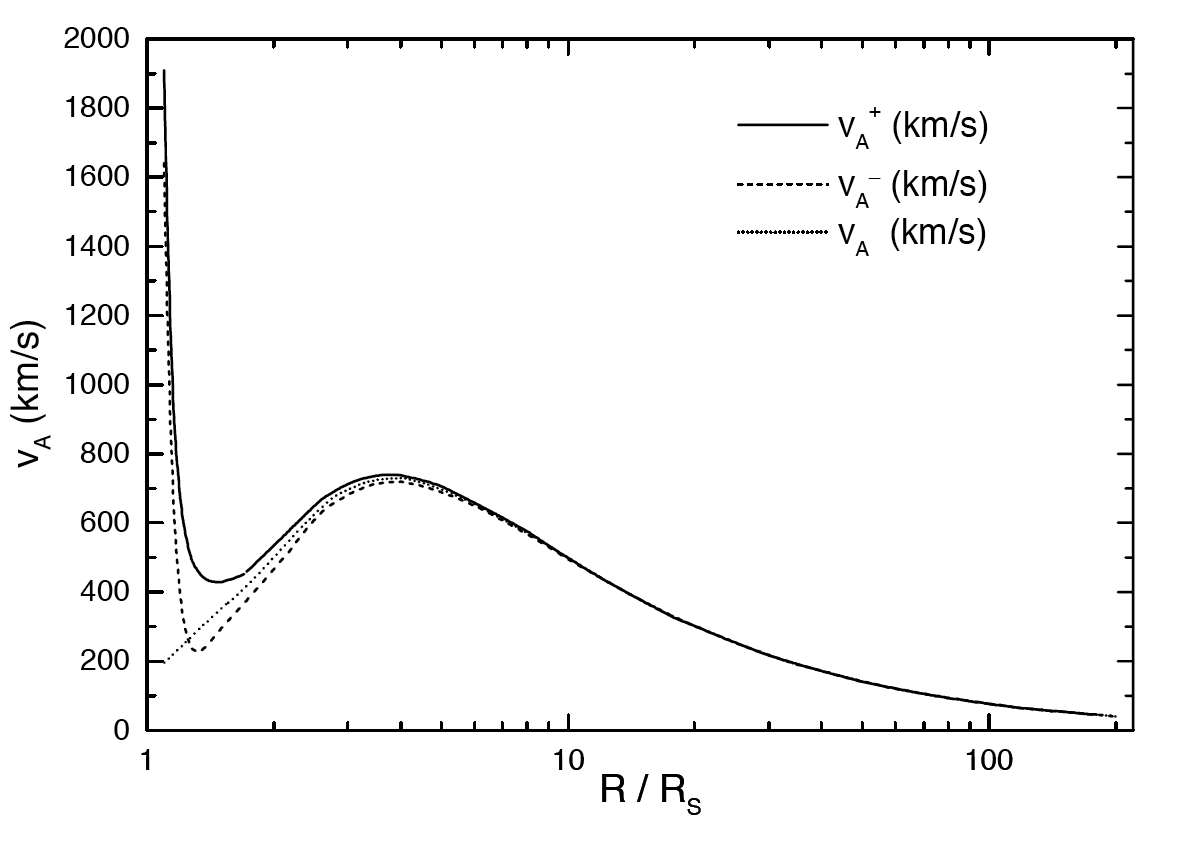
\includegraphics[scale=0.25, trim=0cm 2cm 0cm 2cm]{alfven_speed.png}
\caption[Model of the Aflv\'{e}n speed as a function of height in the corona]{Alfv\'{e}n speed of the corona as a function of heliocentric distance. The dotted line is the quite sun, with only the Sun's global dipole field. The solid line is the Alfv\'{e}n speed calculated from a combination of te global dipole field and a smaller active region dipole field oriented parallel to the global dipole. The dashed line is the the speed when the active region dipole is anti-parallel to the global field. The two profiles from the active region show a distinct minimum in the coronal Alfv\'{e}n speed at $\sim1.5\,R_{\odot}$}
\label{fig:alfven_speed}
\end{center}
\end{figure}
Mann et al. produced a 1D model of the variation of Alv\'{e}n speeds in the quiet and active region corona as a function of height Figure. Warmuth then improved this to a 2D model. It shows that CMEs are well capable of producing plasma hocks in the corona, since they may travel far in excess of the Alfv\'{e}n speed. The theory of plasma shocks and the resulting effects of particle acceleration and plasma emission are discussed in the following sections.


\subsection{MHD Shocks}\label{sec:mhd_shocks}

For acoustic shock waves there are a number of conservation equations that quantify the strength of a shock by relating the upstream gas pressure, density, flow speed, and temperature to their downstream counterparts. Such conservation equations are known as the jump conditions and the shock is considered a surface at which the fluid properties change discontinuously. The shock thickness is usually of the order of a few mean free paths of the particles in the gas, in such a case the processes in the shock surface itself are inconsequential and the relationship between upstream and downstream parameters provide a sufficient description of the shock. 

When the gas is ionized and a magnetic field is present, the jump conditions must be modified to take into account the magnetic pressure and the field orientation with respect to the flow velocity and shock normal $\hat{n}$ (unit vector normal to the shock plane). In the general case of oblique shock waves where the magnetic field direction has some arbitrary angle with respect to shock normal we may derive a set of conservation equations for the frame of the shock wave. 
\begin{figure}[h!]
\begin{center}
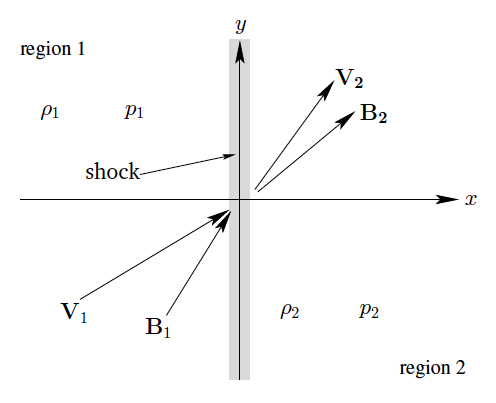
\includegraphics[scale=0.5, angle=0]{images/shock_pic}
\caption[MHD shock framework]{Orientation of magnetic field and velocity field with respect to shock plane, in the rest frame of the shock. Shock normal in this case would be along the $-x$ direction i.e., into upstream region 1. \citep{fitz}}
\label{fig:shock_pic}
\end{center}
\end{figure}

The flow velocity $v$ and magnetic field $B$ are considered to be in the xy-plane. The appropriate conservation  equations are
\begin{subequations}
\begin{align}
&[\rho v_{x}]=0 \\
&[\rho v_{x}^2+p+\dfrac{B_{y}^2}{2\mu}]=0 \\
&[\rho v_{x}v_{y} - \dfrac{B_{x}B_{y}}{\mu}]=0 \\
&[\dfrac{1}{2}v^2 + \dfrac{\gamma p}{(\gamma-1) \rho}+\dfrac{ B_{y}(v_{x}B_{y} - v_{y}B_{x})}{\mu \rho v_{x}} ]=0 \\
&[B_{x}]=0 \\
&[v_{x}B_{y} - v_{y}B_{x}]=0 
\end{align}
\end{subequations}
These are the general MHD shock jump conditions where $v$ is the fluid velocity and $B$ is the magnetic field (with their corresponding components $\textquoteleft$x' or $\textquoteleft$y'), $\rho$ is the mass density, $p$ is the thermal pressure, and $\gamma$ is the ratio of specific heats (or the polytropic index). The meaning of the square brackets is $[F]\equiv F_{1}-F_{2}$, for any quantity F, and the $1$ or $2$ subscripts represent upstream or downstream values of each quantity F, respectively. These set of jump conditions differ only from the purely acoustic ones due the presence of the magnetic field. For example, taking (4a), (4b), and (4d) and setting $B_{x}=B_{y}=0$ we obtain the jump conditions for a neutral gas. Each conservation equation has a specific meaning; 
\begin{itemize}
\item (4a) is a mass conservation equation whereby the mass flux entering the shock must equal the mass flux leaving. It has units of kg\,m$^{-2}$\,s$^{-1}$.
\item (4b) indicates that if mass flux $\rho_{1} v_{x,1}$ enters the shock with momentum $(\rho_{1} v_{x,1})v_{x,1}$ it leaves the shock with momentum $(\rho_{1} v_{x,1})v_{x,2}$, the difference being equal to the the changing force per unit area across the shock. In this case both thermal and magnetic pressures contribute to change in momentum flux. (4c) implies the same process but relates the $x$ and $y$ components of the $v$ and $B$ vector fields. Both equations have units of momentum flux $\equiv$ (kg\,m$^{-2}$\,s$^{-1}$)(m\,s$^{-1}$) = (kg\,m\,s$^{-2}$m$^{-2}$) = N\,m$^{-2}\equiv$ pressure.
\item (4c) is an energy conservation term, accounting for the rate at which gas and magnetic pressure do work per unit area at the shock and equates this to the growth (or loss) in internal energy and kinetic energy across the shock. All components of magnetic field pressure are taken into in the last term on the left of the equation. All quantities are in units of J$\cdot$kg$^{-1}$.
\item (4d) simply states that the x component of the magnetic field i.e., the component of the field that is (anti-)parallel to the shock normal $\hat{n}$ is unaffected by the shock transition. 
\item (4f) relates the orientations of the upstream and downstream magnetic field to the flow speed tangential and perpendicular to the shock normal. Magnetic field orientation and hence the distribution of low speed amongst the velocity components largely depends on the whether the shock is slow-mode, intermediate, or fast mode. The equation has units of T$\cdot$m$\cdot$s$^{-1}$ = V$\cdot$m$^{-1}\equiv$ electric field.
\end{itemize}

4(a-f) are the general case of the jump conditions across an MHD shock, they are usually known as the MHD Rankine-Hugoniot (RH) equations. Their generality make the solution of the six unknowns from the six equations quite complicated. However the extreme cases of parallel and perpendicular shocks provide very useful and simplified expressions. It can be shown that parallel shocks i.e., $\hat{v}\parallel\hat{B}\parallel\hat{n}$ reduces to the jump conditions of a hydrodynamic shock in a neutral gas (here parallel and anti-parallel are used synonymously). The more interesting case when considering radiating shockwaves in the low solar corona is the perpendicular (or quasi-perpendicular) MHD shock, in this case the flow speed is parallel to the shock normal, and the magnetic field is perpendicular (or at a high angle) to it i.e., $\hat{v}\,\|\,\hat{n}$ and $\hat{B}\perp\hat{n}$. As will be shown it is this special case of quasi-perpendicular shocks that lead to efficient shock drift particle acceleration, a necessary precursor to the generation of radio emission at a coronal shockwave. 

In the case of fully $\perp$ shocks there is no need for the decomposition of the magnetic and velocity vector fields, meaning the $x$ and $y$ subscripts on 4(a) and 4(b) can be dropped. 4(c) is an obsolete jump condition, likewise for 4(e) since no $B_x$ field exists. We can also rid the $B_{x}B_{y}$ terms from the last quotient in the energy conservation 4(d) --replacing it simply with $B^{2}/2\mu\rho$. 4(f) reduces to a simpler form of $[Bv]=0$. Such a reduction in the generalized jump conditions allows us to express the upstream and downstream plasma properties in terms of the shock compression ratio $\chi=\dfrac{\rho_{2}}{\rho_{1}}$ as well as the upstream sonic Mach number $M_{1}=\dfrac{v_{1}}{c_{1}}$ \citep{priest2000} e.g.,
\begin{subequations}
\begin{align}
&\dfrac{v_{2}}{v_{1}}=\frac{1}{\chi} \\
&\dfrac{B_{2}}{B_{1}}=\chi \\
&\dfrac{p_{2}}{p{1}}=\gamma M_{1}^2\bigg(1-\frac{1}{\chi}\bigg) - \frac{1-\chi^2}{\beta_{1}}
\end{align}
\end{subequations}
where $\beta_{1}=2\mu p/B_{1}^2$ is the upstream plasma beta parameter. The exact value of the compression ratio may be obtained by using 4(b) to eliminate $p$ from the energy flux equation 4(d) and incorporating 4(a,c,e,f) (and a lot of algebra) a quadratic for $\chi$ may be obtained
\begin{equation}
2(2-\gamma)\chi^{2}+[2\beta_{1}+(\gamma-1)\beta_{1}M_{1}^2+2]\gamma\chi - \gamma(\gamma+1)\beta_{1}M_{1}^2=0
\end{equation}
%where $M_{1}$ is the upstream sonic Mach number, $\beta_{1}$ is the upstream beta parameter and, and $\gamma$ is the ploytropic index. 
Equation (6) has one positive real root such that 
\begin{equation}
1< \chi < \frac{\gamma+1}{\gamma-1}
\label{eqn:compression}
\end{equation}
Using a ploytropic index of $\gamma=5/3$ (monatomic) means the shock compression can be no more than a factor of 4. Another extremely important fact arising from this is that magnetic compression can also be no greater than 4 i.e., from equation 4(b) $B_{2}/B_{1}=\chi$. $\chi<4$ has consequences for the shock drift acceleration mechanism and provides an upper limit to the particle energy gain.

\subsection{Shock Particle Acceleration}\label{sec:30}

The framework of shock particle acceleration for solar type II radio bursts is called the shock drift acceleration (SDA) mechanism \citep{holman1983}. The mechanism involves a gyrating particle encountering the magnetic gradient caused by the shock, resulting in a guide center drift and an energy gain due to the presence of a convective electric field at the shock. 

There are two important frames of reference through which SDA is studied. In the rest frame of the shock, known as the \textquoteleft normal incidence frame' (NIF), the upstream plasma has velocity $\mathbf{u}_1$ along the normal $\hat{n}$ to the shock front. The upstream magnetic field $\mathbf{B}_1$ creates an angle $\theta_{Bn}$ with the shock normal $\hat{n}$, and the downstream counterparts have values $\mathbf{u}_2$ and $\mathbf{B}_2$, Figure~\ref{fig:nif_dht}(left). 

\begin{figure}[!t] 
\begin{center}
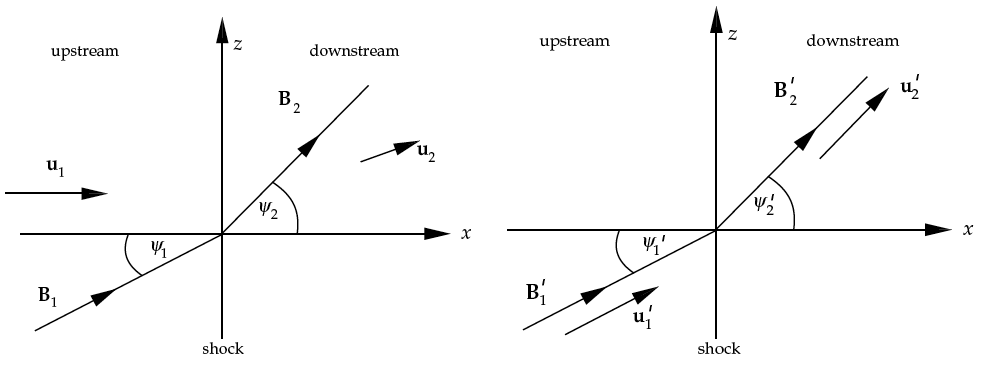
\includegraphics[scale=0.45]{nif_dht}
\caption[Normal incidence and de Hoffman-Teller reference frames]{(Left) Normal incidence frame (NIF) where the shock is at rest and the upstream plamsa approaches the shock head-on at velocity $\mathbf{u}_1$. The magnetic field makes some arbitrary angle $\theta_{Bn}$ with the shock normal. (Right) Transformation to a de Hoffman-Teller frame ensures that the plasma velocity and magnetic field are in the same direction on both sides of the shock \citep{ball2001}.}
\label{fig:nif_dht}
\end{center}
\end{figure}

Due to the motion of the plasma across the magnetic field, there is a convective electric field given by $\mathbf{E} = \mathbf{v}\times \mathbf{B}$, which causes a drift of the particles with speed $\mathbf{v}_E = \mathbf{E}\times \mathbf{B}/B^2$. The kinematics of the particle in the shock drift acceleration mechanism are best treated in a frame where there the convective electric field vanishes such that $\mathbf{E} = |\mathbf{v}\times \mathbf{B}|=v_x B_y - v_yB_x = 0$. The frame where this criterion is fulfilled is known as the de Hoffmann-Teller frame (dHTf) \citep{dehoffmann1950} and has a frame velocity with respect to the NIF frame given by. 
\begin{equation}
v_{HT} = v_y = u_1\mathrm{tan}\theta_{Bn}
\end{equation}
This frame guarantees the plasma motion is in the same direction as the magnetic field on both sides of the shock. Given the absence of any electric fields in this frame, the particle motions may be treated as having a conserved magnetic moment \citep{ball2001}
\begin{equation}
\mu = \frac{mv^2_{1\perp}}{B_1} = \frac{mv^2_{2\perp}}{B_2} = \mathrm{const}
\label{eqn:ad_in}
\end{equation}
where the subscripts [1,2] represent pre an post-encounter shock values respectively. In the dHTf, the conservation of the magnetic moment may be used to derive the particle kinematics given either reflection or transmission though the shock. Rearrangement of equation \label{eqn:ad_in} shows that particles with a pitch angle fulfilling the relationship
\begin{equation}
\alpha > \alpha_c~~~~\mathrm{where}~~~~\mathrm{sin}^2\alpha_c = \frac{B_1}{B_2}
\end{equation}
will be reflected at the shock. This pitch angle $\alpha_c$ defines a \textquoteleft loss-cone' in velocity space $f(v_{\perp}, v_{||})$, whereby any particle within the cone (large $v_{||}$) will be lost downstream, while particles outside the loss cone will be reflected at the shock. This is known as a \textquoteleft magnetic mirroring', a process that shocks are known to exhibit \citep{feldman1983}. Inside the dHT reference frame, the particles energy (whether reflected or transmitted) is completely conserved and there is no energy gain. Conceptually, the best way to see where the acceleration takes place is in the normal indcidence frame (NIF).

In the NIF, the particles gyrate about the upstream magnetic field $\mathbf{B}_1$, while there is a convective electric causes a small drift of magnitude $\mathbf{v}_E = \mathbf{E}\times \mathbf{B}/B^2$ towards the shock. If the particle speed is much greater than the shock speed $v>>u$, the particle undergoes many Larmor gyrations while in contact with the shock. The difference between the Larmor radius of the orbit ahead of and behind the shock front (due to the increased downstream magnetic field) will cause the particle to drift parallel to the shock surface \citep{ball2001, toptychin1980}, Figure~\ref{fig:sda}. This is equivalent to a \textquoteleft grad-B' drift in an inhomogeneous magnetic field. This drift allows a charged particle to move parallel to the convective electric field, allowing the E-field to do positive work on the particle and produce an energy increase. Overall, a grad-B drift at the shock surface gives the particle a component of velocity that may interact with the convective electric field, hence the process is known as \textquoteleft drift-acceleration'.

\begin{figure}[!t] 
\begin{center}
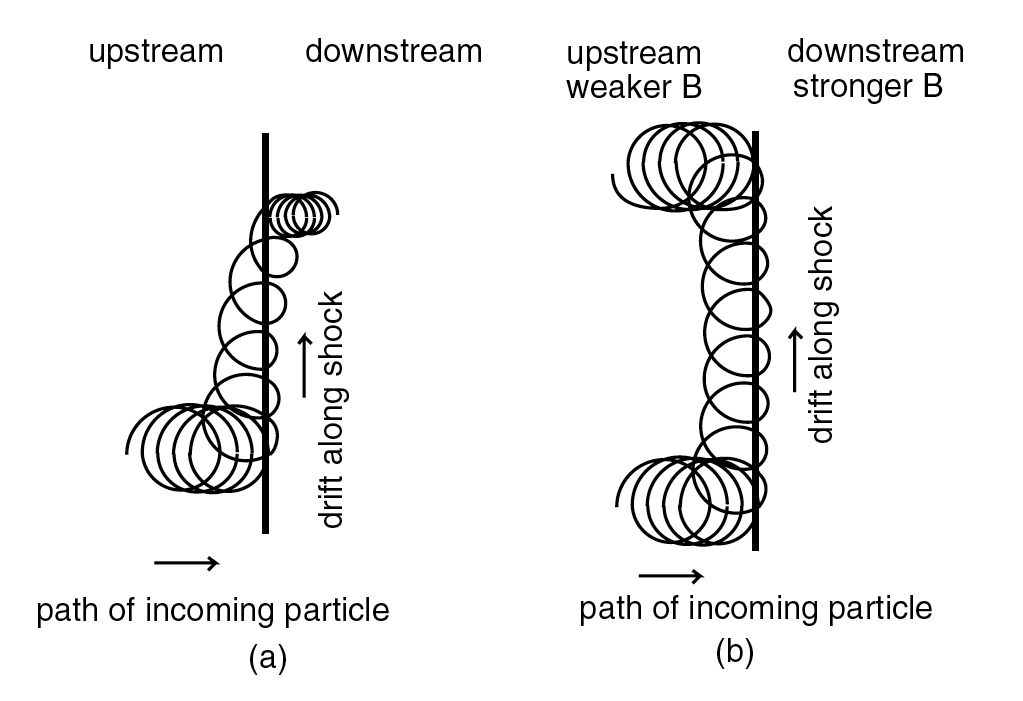
\includegraphics[scale=0.3]{sda_original}
\caption[Shock drift acceleration]{Particle drift paths due during both a transmitted (a) and reflected (b) motion. The increased magnetic field in the downstream region caused a drift along the surface. This drift occurs in the presence of a convective electric field (which will have a component parallel to the drift), allowing the field to do work on the particle and hence increase its energy \citep{ball2001}.}
\label{fig:sda}
\end{center}
\end{figure}

While the energy gain is most apparent in the NIF frame, particle reflection and transmission is best handled mathematically in the dHT frame. Hence firstly, the magnetic mirroring process is described in dHT, while the post-encounter speed and energy gain are then obtained by converting back to the rest frame of the upstream plasma (NIF). Reference has shown that the particle energy gain upon reflection from the shock is given by 

\begin{equation}
\frac{E_r}{E_i} = \frac{1+\sqrt{1-B_1/B_2}}{1-\sqrt{1-B_1/B_2}}
%v^r_{||} = 2u_1\mathrm{sec}\theta_1 - v^i_{||}
\end{equation}
The energy gain is limited to the magnetic field strength jump across the shock, and since this field strength is limited by equation~\ref{eqn:compression}, the energy gain is limited to a factor of 13.93 \citep{ball2001}. A similar treatment may also give the reflected velocity in terms of the incident velocity \citep{holman1983}
\begin{equation}
v^r_{||} = 2u_1\mathrm{sec}\theta_1 - v^i_{||}
\end{equation}
shock drift acceleration has been used to explain the presence of $1-100$\,keV electron at Earth's magnetospheric bow shock \citep{wu1984}, in the context of radio bursts have used it to explain the acceleration of electrons during type II and herringbone bursts \citep{holman1983, mann2005, schmidt2012b}
More sophisticated models involve multiple reflections at the shock that increase the energy gain each time, thereby producing energies that are observed in the vicinity of shocks. This multiple reflection process plays an important role in some theoretical treatments of herringbone emission; we will return to this point in Chapter 5.



\subsection{Wave-Particle Interaction}\label{sec:wave_particle}

%Distributions of particles in a plasma can give rise to resonances in various wave modes. In general we may relate a particle distribution function in velocity space $f(v_{\|})$ with a distribution function of wave modes in wave-number or $\textquoteleft\mathbf{k}$-space' $N(\mathbf{k})$
%\begin{equation}
%\frac{\partial N(\mathbf{k})}{\partial t}+v_{g}(\mathbf{k})\frac{\partial N(\mathbf{k})}{\partial r} = \Gamma(\mathbf{k},f(v_{\|}))N(\mathbf{k})
%-\Gamma_{coll}(\mathbf{k}) N(\mathbf{k})
%\end{equation}
%where the lefthand side takes the form of a Lagrangian derivative with group speed $v_g$, $\Gamma$ represents a wave growth term given the distribution function $f(v_{\|})$, and $\Gamma_{coll}$ is a term taking into account collisional damping of the wave \citep{aschbook}.

The treatment of the interaction of particles and waves in a plasma is in determining what the oscillatory response of a plasma is to a velocity distribution function \citep{inan2011}. In order to see how the distribution function effects wave growth we start with an equilibrium distribution $f_0$ and impose a perturbation $f_1(\mathbf{r}, \mathbf{v}, t)$, so that the total distribution function is $f(\mathbf{r}, \mathbf{v}, t) = f_0 +f_1(\mathbf{r}, \mathbf{v}, t)$.  The perturbation quantities will take the form $e^{i(\omega t + \mathbf{k}r)}$ i.e., perturbation quantities that are periodic in space and time with eave number $\mathbf{k}$ and angular frequency $\omega$.

To see how $f(\mathbf{r}, \mathbf{v}, t)$ evolves in time we insert it into the Vlasov equation and linearize, ignoring any terms higher than second order
\begin{equation}
\frac{\partial f_1}{\partial t} + (\mathbf{v}\cdot \nabla)f_1 +\frac{q_e}{m_e}(\mathbf{E} + \mathbf{v}\times \mathbf{B})\cdot\nabla_vf_0=0
\end{equation}
%Assuming an isotropic $f_0$ it can be shown that $(\mathbf{v}\times \mathbf{B})\cdot\nabla_vf_0=0$, and 
Using Poisson's equation (Maxwell first equation) and replacing the time and space derivatives with their oscillatory operators ($\partial/\partial t \rightarrow -i\omega$, $\nabla \rightarrow i\mathbf{k}$), the perturbed Vlasov equation may be rearranged to give
\begin{equation}
f_1=\frac{q_e}{m_e}\frac{j}{\omega-\mathbf{k\cdot v}}\mathbf{E}\cdot\nabla_vf_0
\label{eqn:f_pert}
\end{equation}
This equation relates the perturbed quantity $f_1$ to the unperturbed distribution function and the electric field. The most important aspect of this equation is the $\omega-\mathbf{k\cdot v}$ term in the denominator, implying the possibility of resonance. Now, integrating both sides of \ref{eqn:f_pert} over all velocity space and again using Poisson's equation results in
%using (19) the general form of the dispersion relation of the oscillations $(\omega,\mathbf{k})$ in perturbations $f_1$ and $E$ is derived
\begin{equation}
1+\frac{q_e}{\epsilon_0m_e}\frac{1}{k^2}\mathbf{k}\cdot\int_v\frac{\nabla_v f_0}{\omega-\mathbf{k\cdot v}}d^3v=0
\label{eqn:dispersion}
\end{equation}
Any electrostatic normal mode oscillations satisfy this relationship and integrating over all velocity space will result in a dispersion relation for the oscillations of the plasma property $f_1$. The equation effectively gives the oscillatory response $\omega = g(\mathbf{k})$ of the perturbation $f_1$ of the plasma, given a particular velocity distribution function $f_0$. For example, a cold plasma distribution function where $f_0 = N_0\delta(\mathbf{v})$, where $\delta$ is a dirac-delta, in equation~\ref{eqn:dispersion} will result in a dispersion relation of
\begin{equation}
1 - \frac{N_0q_e^2}{\epsilon_0 m_e \omega^2} = 0 
\end{equation}
The perturbed Vlasov equation with a cold plasma model (no thermal motions) produces the expression for a plasma oscillation. The integral over velocity space in this case can be performed because the delta function guarantees that there is no velocity with the property of $v = \frac{\omega}{\mathbf{k}}$. If this were to be fulfilled, there is the possibility of resonances equation~\ref{eqn:dispersion} i.e., the integral is non-trivial as $v \rightarrow \frac{\omega}{k}$. This states that if there are electrons in the particle distribution function that match the phase speed of oscillations in the plasma then the integral will have a singularity or 'pole'. To avoid the singularity producing unphysical results, the integration is performed in complex space using a method called contour integration \citep{melrose1989}. The use of contour integration means there will be complex solutions of the dispersion relation of the form $\omega = \omega_r + i\gamma$.
The real part of the solution applies as normal where the integral is well behaved, far from the singularity. However, integration over the singularity necessitates a complex solution (from the contour integration), hence the $\omega$ consists of both real and imaginary parts.
The complex $i\gamma$ means that a time dependency of the periodic solutions to the perturbations $f_1$ will be 
\begin{equation}
e^{j\omega t}=e^{(i[\omega_r + i\gamma])}=e^{i\omega_rt}e^{-\gamma t}
\end{equation}
This solution is a damped wave with damping factor $\gamma$, meaning the solution to equation~\ref{eqn:dispersion} in the region $v \sim \omega/k$ provides a wave decay term. These are the essential elements of Landau damping e.g., if the phase speed of the waves in a plasma match the speed of electrons in the distribution function then those waves will experience a damping. However, the damping term is dependent on the negative of the velocity space gradient at $v=\frac{\omega}{k}$ \citep{melrose1989}
\begin{equation}
\gamma \sim -\nabla_v f_0|_{v=\frac{\omega}{k}}
\end{equation}
If there are a group of electrons that have the same speed of a particular wave in the plasma they may exchange energy with this wave efficiently. If there is a negative gradient on the velocity distribution at $v=\frac{\omega}{k}$, this will lead to wave damping. However, a positive gradient in the velocity distribution will result in $\gamma <0$ and a wave growth term that increases exponentially. Effectively, %if a group of electrons is promoted to a speed that matches the phase speed of Langmuir waves in the plasma, and their velocity space gradient at the phase speed is positive, then Langmuir waves will grow exponential. This group of electrons is called a bump-on-tail, since it is described by a Gaussian bump on the high velocity tail of a Maxwell distribution function. The growth of Langmuir waves in a resonant response to this beam is called the bump-on-tail instability.
a group of electrons is promoted to a velocity range that closely matches the phase speed of some type of waves in a medium $v \sim \omega/k$. In such a speed range the integrand of (equation) approaches the point at which there is a singularity in the solution. Such a point necessitates a complex solution to the integral, thus providing an imaginary part to the dispersion relation that gives an $e^{-\gamma t}$ term. If the promotion of electrons to a range $v \sim \omega/k$ is combined with a positive gradient of the distribution function in this velocity range, it results in $\gamma < 0$ and $e^{-\gamma t}>0$, leading to wave growth. This is why $v - \omega/k=0$
is known as the resonance condition \citep{melrose1989}. Since electron beams in the corona match the phase speed of Langmuir waves, the beam results in the generation of Langmuir waves. This group of electrons in the beam is called a bump-on-tail, since it is described by a Gaussian bump on the high velocity tail of a Maxwell-Boltzmann velocity distribution function (Figure~\ref{fig:bot}). 
\begin{figure}[!t] 
\begin{center}
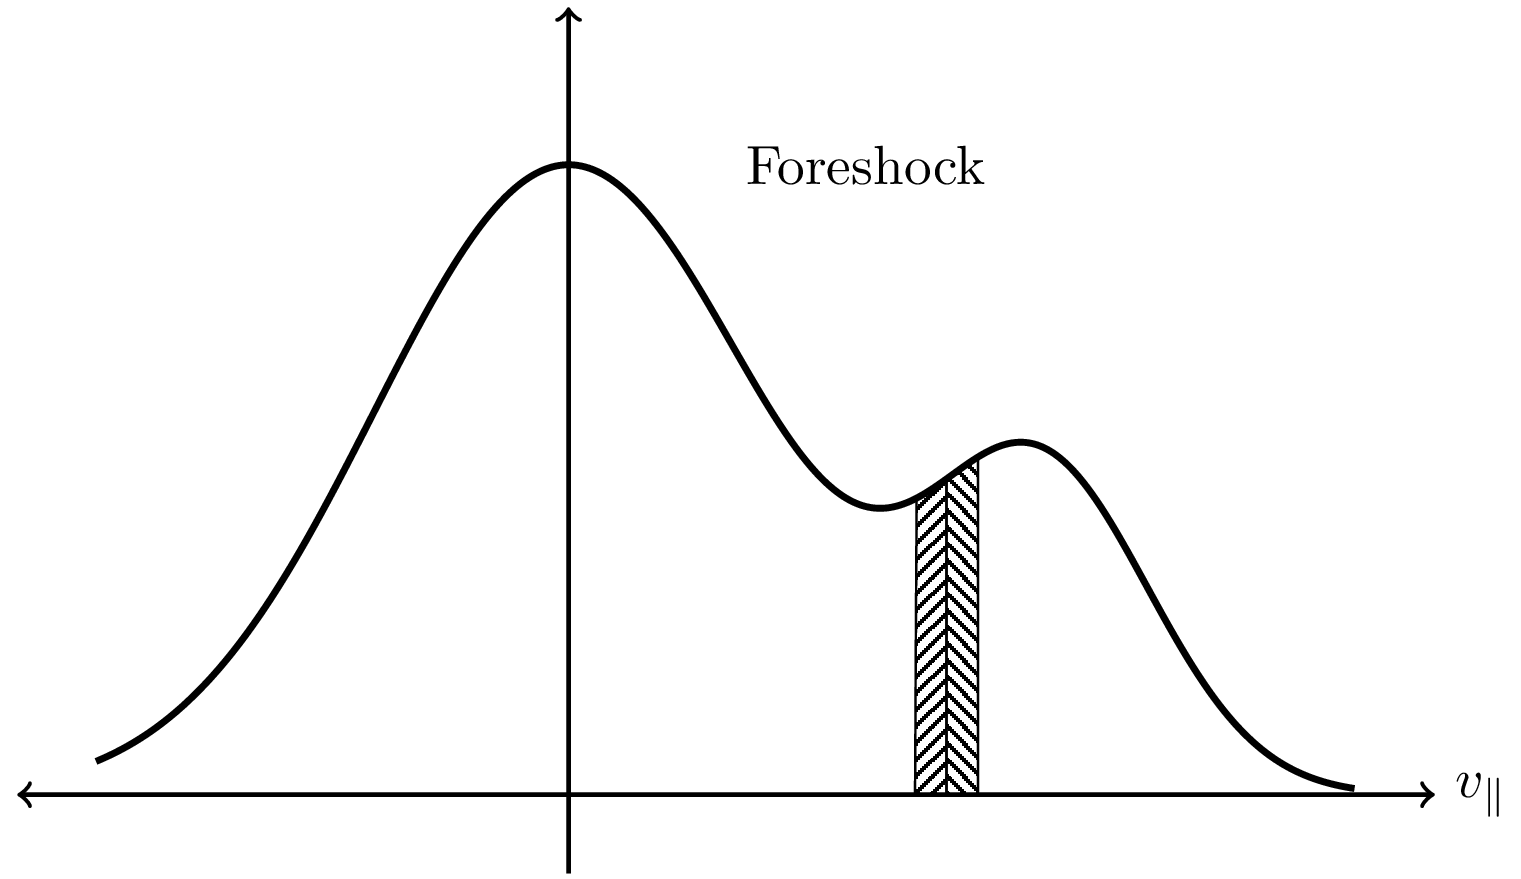
\includegraphics[scale=0.2]{bump_on_tail}
\caption[Shock drift acceleration]{Maxwell-Boltzmann velocity distribution with a Guassian `bump-on-tail' representing the beam. The shaded region are those electrons that will produce a bump-on-tail instability due to the presence of a positive slope in the distribution function.}
\label{fig:bot}
\end{center}
\end{figure}
The growth of Langmuir waves in a resonant response to this beam is called the bump-on-tail instability. Once these Langmuir waves are generated they may undergo decay or coalescence with other waves to produce electromagnetic radiation. 

%\begin{figure}[!t]
%\begin{center}
%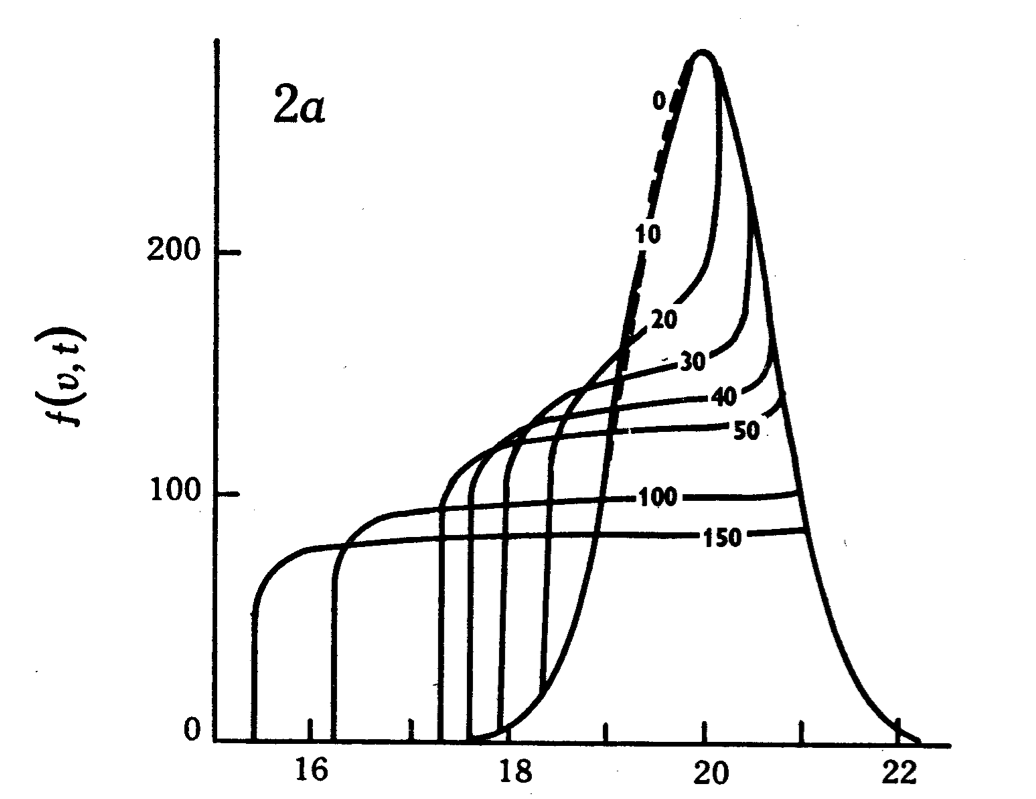
\includegraphics[scale=0.35, trim = 4cm 0cm 0cm 0cm]{images/Grognard1975}
%\end{center}
%\end{figure}


\subsection{Three-Wave Interaction and Plasma Emission}\label{sec:three_wave}

Once the Langmuir waves are produced from the bump-on-tail instability a number of wave interaction processes occur in order to bring about plasma emission. This involves the interaction of various wave modes in the plasma described by a mathematical formalism called the three-wave interaction \citep{robinson1993, robinson1994}. In this process three wave modes in a plasma M, P, and Q are described by their distribution functions in a wave-number space ($k$-space). the distribution functions are given by $N_M(k_M)$, $N_P(k_P)$, $N_Q(k_Q)$, where the $N$ describe the occupation number of wave quanta between $k$ and $k+dk$ in the wave-number space. Waves in P and Q mode may interact to such that wave quanta are removed from the P and Q k-space and added to the M k-space. This is essentially an emission of an energy packet from the P and Q -space to the M k-space. The rate of change of occupation numbers in the three k-spaces are given by
\begin{eqnarray}
\frac{dN_M(\mathbf{k}_M)}{dt} = -\int \frac{d^3\mathbf{k}_P}{(2\pi)^3}\int \frac{d^3\mathbf{k}_Q}{(2\pi)^3}g(\mathbf{k}_M, \mathbf{k}_P, \mathbf{k}_Q) \\
%
\frac{dN_P(\mathbf{k}_P)}{dt} = -\int \frac{d^3\mathbf{k}_M}{(2\pi)^3}\int \frac{d^3\mathbf{k}_Q}{(2\pi)^3}g(\mathbf{k}_M, \mathbf{k}_P, \mathbf{k}_Q) \\
%
\frac{dN_Q(\mathbf{k}_Q)}{dt} = -\int \frac{d^3\mathbf{k}_M}{(2\pi)^3}\int \frac{d^3\mathbf{k}_P}{(2\pi)^3}g(\mathbf{k}_M, \mathbf{k}_P, \mathbf{k}_Q)
\end{eqnarray}
where $g(\bf{k}_M, \bf{k}_P, \bf{k}_Q)$ is an expression that incorporates a transition probability for wave quanta into and out of energy states in the various k-spaces \citep{robinson1994}. The transition probability of waves amongst states M, P and Q is given by \citep{melrose1986}
\begin{equation}
u_{MPQ}(\mathbf{k}_M, \mathbf{k}_P, \mathbf{k}_Q)  \propto \delta(\omega_M - \omega_P - \omega_Q ) \delta^3(\mathbf{k}_M - \mathbf{k}_P - \mathbf{k}_Q )
\end{equation}
where the $\omega$ are the frequency of the corresponding wave and and $\delta$ are delta functions. This is analogous to transition probabilities given by the Einstein coefficients for transferring energy packets from and atomic state to a photon state (photon emission) i.e., whereas the Einstein coefficients are used in atom-wave (atom-photon) energy exchanges, $u_{MPQ}$ describes wave-wave energy exchanges. Given the presence of delta functions in the transition probability expression, we can see that an exchange of energy quanta amongst the wave modes can only occur when 
\begin{eqnarray}
\omega_M & = & \omega_P + \omega_Q \\
\mathbf{k}_M & = & \mathbf{k}_P + \mathbf{k}_Q
\end{eqnarray}
Hence for an a conversion wave modes in a plasma such as $M \rightarrow P + Q$ (a decay of mode M into P and Q), or it's reverse process $P + Q \rightarrow M $ (a coupling of P and Q to produce M) is described by equations (2.1) to (2.7). 

%\begin{multline}
%g(\mathbf{k}_M, \mathbf{k}_P, \mathbf{k}_Q) = u_{MPQ}(\mathbf{k}_M, \mathbf{k}_P, \mathbf{k}_Q)   [N_M(\mathbf{k_M}) N_P(\mathbf{k_P})  - \\ 
%N_P(\mathbf{k_P}) N_Q(\mathbf{k_Q})   +N_Q(\mathbf{k_Q}) N_M(\mathbf{k_M})  ]
%\end{multline}
%where $u_{MPQ}(\bf{k}_M, \bf{k}_P, \bf{k}_Q) $ is the transition probability from states in P and Q  to M, for example \citep{melrose1986}.  The transition probability is given by

%where the $\omega$ are the frequency of the corresponding wave and and $\delta$ are delta functions. 
The production of plasma emission after a bump-on-tail instability has occurred requires a three wave interaction amongst a Langmuir wave $L$, ion acoustic wave $S$, and electromagnetic wave $T$. Fundamental emission during a radio burst occurs via a decay of Langmuir waves into an electromagnetic and ion sound wave
\begin{equation}
L \rightarrow T + S
\label{eqn:fund}
\end{equation}
while second harmonic first requires the decay $L\rightarrow L^{'} + S$, where $L^{'}$ is a product Langmuir wave propagating in the opposite direction to the first. This is followed by a coalescence of the original and product Langmuir waves
\begin{equation}
L + L^{'}\rightarrow T'
\label{eqn:harm}
\end{equation}
In the case of these three interacting waves then 
\begin{eqnarray}
\omega_T & = & \omega_L + \omega_S \\
\omega_{T^{'}} & = & \omega_L + \omega_{L^{'}}
\end{eqnarray}
where the relevant dispersion relations are 
\begin{eqnarray}
\omega_L = \omega_p + \frac{3v_{th}^2}{2\omega_p}k_L^2 \\
\omega_T = (\omega_p^2 +k_T^2c^2)^{1/2} \\
\omega_S = k_s\sqrt{\frac{\gamma k_B T_e}{m_i}}
\end{eqnarray}
where
\begin{equation}
\omega_p = \bigg(\frac{n_e e^2}{m_e \epsilon_0}\bigg)^\frac{1}{2}
\label{eqn:plasma_frequency}
\end{equation}
These equations imply that when a Langmuir wave decays to an electromagnetic wave and an ion sound wave (equation 2.58), the frequency of the electromagnetic wave will be equal to that of the Langmuir wave such that $\omega_T = \omega_L \approx \omega_p$. This is why plasma emission occurs at the local plasma frequency. Similarly the production of $T^{'}$ via equation (2.59) results in the first harmonic $\omega_T \approx 2\omega_p$. 
%!!!!!!!!!!!!!!!!!!!!!!!!!!!!!
%
%PROVE THE ABOVE MORE CLEARLY!!!!!!!!!!!!!!!!!!!!!!
%
%!!!!!!!!!!!!!!!!!!!!!!!!!!!!

In order to investigate the amount of energy emitted by the electromagnetic wave, elements of the three wave interaction theory need to be combined with what is known as stochastic growth theory \citep{robinson1993a}(SGT). Stochastic growth theory was first developed in response to a number of criticisms of the theory of a beam-driven Langmuir wave hypothesis of type III radio bursts first proposed by \citet{ginzburg1958}. It was pointed out that if the beam was to remain in instability continuously over space and time in the absence of saturation mechanism, then it would quickly lose all of its energy to the Langmuir waves and consequently the beam electrons would stop propagating after a short distance \citep{sturrock1964}. This is clearly not the case, since type III electrons are observed to propagate over distances of 1\,A.U or more. 
%Secondly, if the instability continues uninhibited the Langmuir wave with grow to levels far beyond what is observed \citep{smith1979}. 
%It was concluded that the beam cannot remain in a state of instability for the duration of its propagation. One suggestion to over come this was quasi-linear relaxation \citep{grognard1975}, as described above. However, this may not be enough to guarantee a lone lifetime of the beam. 
SGT overcomes this by describing an electron beam propagation in a state of marginal stability. The beam propagates in an inhomogeneous medium whereby it encounters pockets of localised density enhancement where it is unstable intermittently. As the beam propagates through this localised clump, it is unstable to the growth of Langmuir wave, giving up some of its energy to the wave, diminishing the beam slightly. Once it exits the clump it becomes stable again, allowing the beam to reform until it reaches another localised clump to give up some energy again. The Langmuir waves would then experience a growth at intermittent regions in space and time (which is actually observed \citep{lin1986}), while the beam would be unstable for only small fractions of its lifetime. Overall, the beam energy loss is on average low enough to allow its continued propagation, but instantaneous and finite enough to allow the growth of waves. 
%In this mechanism the Langmuir waves experience a a growth in energy that is a random (stochastic) walk through energy phase space \citep{robinson1992}.  The Langmuir wave send up with an energy distribution given by $P(E)\sim E^{-1}$ \citep{robinson1993a}.  
\begin{figure}[t!]
\begin{center}
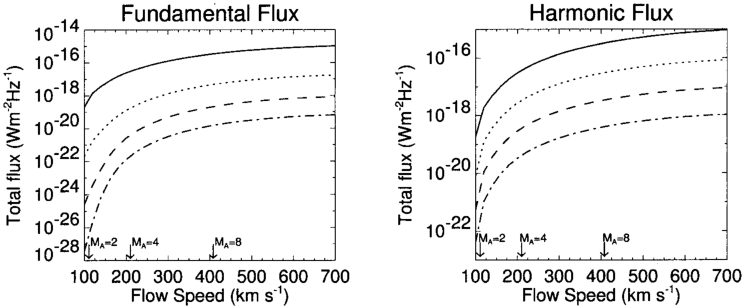
\includegraphics[scale=1.1, trim=0cm 0cm 0cm 0.5cm]{images/Cairns2003.pdf}
\caption[Theoretically predicted radio burst fluxes]{Theoretical flux of the fundamental and harmonic emission bands of a type II radio burst using three wave interaction and stochastic growth theory \citet{cairns2003}.}
\label{fig:cairns_emissivity}
\end{center}
\end{figure}
Combining elements of the stochastic growth model and the three-wave interaction process allows a calculation of the mount of energy that ends up in the electromagnetic waves, and consequently the volume emissivity of the emission \citep{robinson1993a, robinson1998}
\begin{equation}
j_M(r) \approx \frac{\Phi_M}{\Delta\Omega_M}\frac{n_b m_e v_b^3}{3l(r)}\frac{\Delta v_b}{v_b}
\end{equation}
here the $M$ stands for either fundamental $F$ or harmonic $H$ emission. $\Delta\Omega_M$ is the solid angle over which the  emission is spread, $n_b$ is the electron beam number density, $v_b$ is the beam speed, $l(r)$ is the distance from emission point to observer, $\Delta v_b$ is the width of the beam in velocity space. $\Phi_M$ are known as the conversion efficiencies and are different for fundamental and harmonic emission, see Appendix X.

These expressions have been used to simulate radio burst flux resulting in $\sim10^{-17}$\,W\,m$^{-2}$\,Hz$^{-1}$, which have been compared to type II and III radio bursts \citep{schmidt2012, knock2001}. \citet{knock2003} and \citet{cairns2003} used the theory to predict interplanetary type II burst flux as a function of a variety of shock parameters e.g., shocks speed Fig.~\ref{fig:cairns_emissivity}.

The theory outlined in section~\ref{sec:mhd_shocks} -- \ref{sec:three_wave} was employed in a model developed by \citet{schmidt2012b}, completely describing the generation of radio bursts from CME driven shocks. It involves the eruption of a flux rope into a background corona, the driving of a shock as described by the MHD Rankine-Hugoniot relations, the generation of electron beams via SDA, the growth of the bump-on-tail instability, and the generation of electromagnetic emission via the three-wave process and stochastic growth theory. The model finds that that radio emission is generated on the expanding flanks of a CME. The model also shows that when the shock is rippled, there will be spatially intermittent regions of electron beam generation, which could be possible explanation of herringbone emission (Figure~\ref{fig:herbone_model}).
% as shown in Figure~\ref{fig:schmidt_model}
%\begin{figure}[t!]
%\begin{center}
%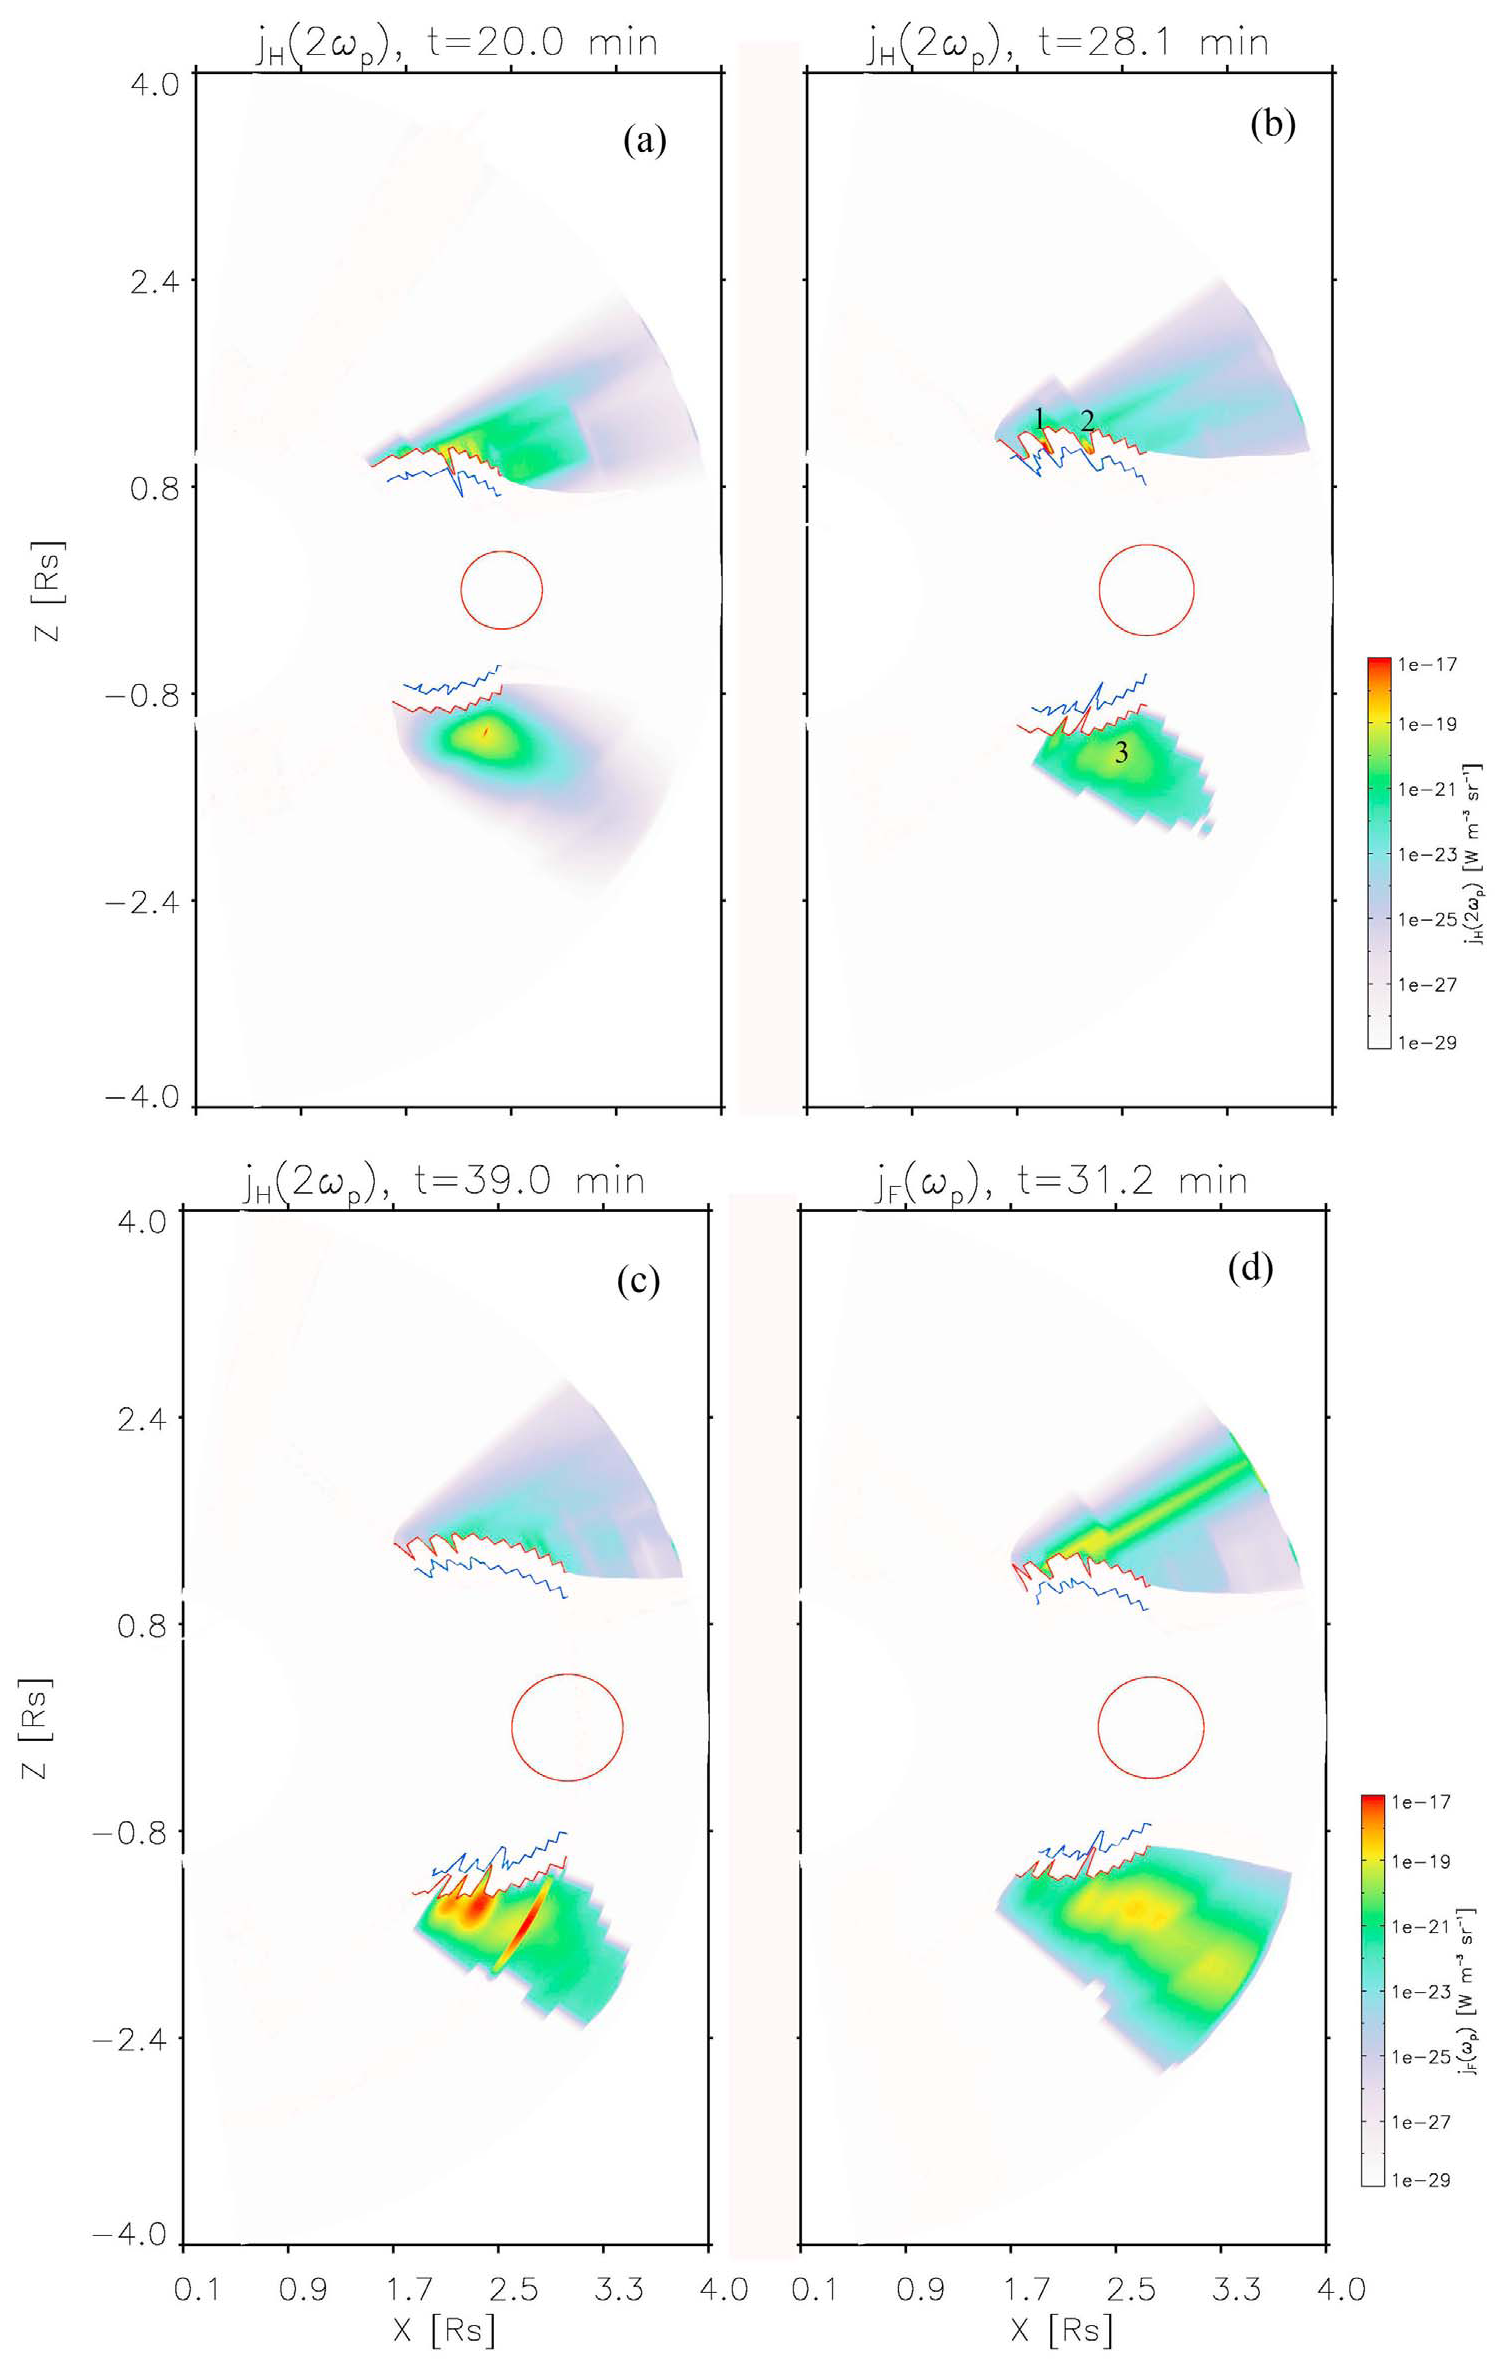
\includegraphics[scale=0.7]{schmidt_model}
%\caption[Model of radio burst driven by expanding CME flanks]{Complete model of radio burst driven by expanding CME flanks}
%\label{fig:schmidt_model}
%\end{center}
%\end{figure}
\begin{figure}[t!]
\begin{center}
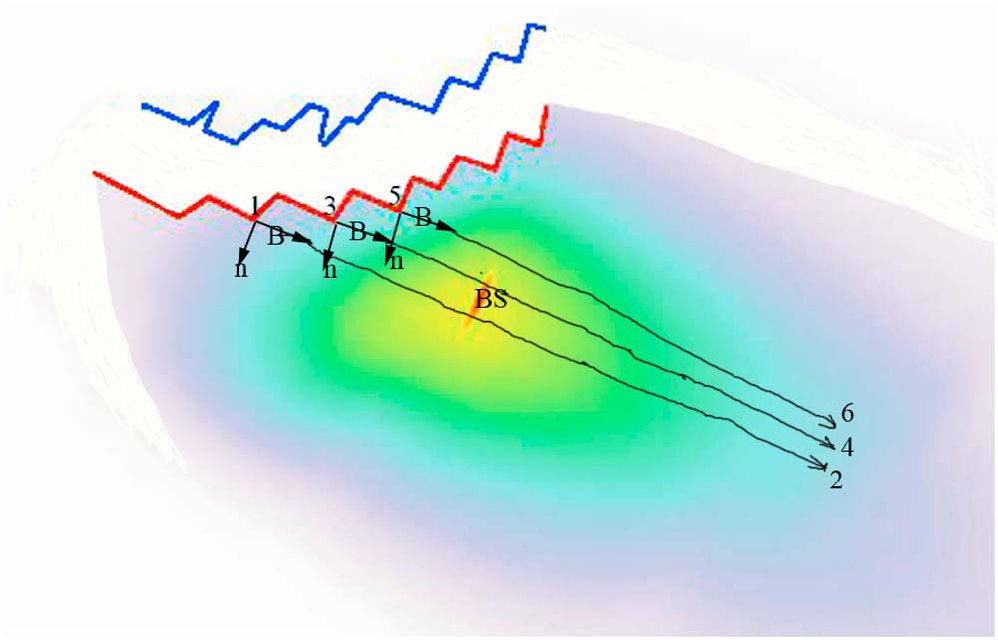
\includegraphics[scale=1.2]{herbone_model}
\caption[Model of radio burst driven by expanding CME flanks]{Model of the radio emission driven by electron beams on the flank of a CME. Each arrow marks the trajectory of the electron beams accelerated at the rippled shock surface. The red and blue lines outline the shock ramp. The green-red colours show radio emission intensity.}
\label{fig:herbone_model}
\end{center}
\end{figure}


\subsection{Frequency Drift of Radio Bursts}\label{sec:freq_drift}

In the previous section it was shown that when plasma emission is excited in the corona, the frequency of emission is close to the plasma oscillation frequency given by equation~\ref{eqn:plasma_frequency}
%As mentioned in section X, the frequency of emission allows a direct conversion from frequency to electron density of the environment in which the emission is generated. Since electron number density in the corona generally varies with height, it is then possible to calculate the height from which this frequency of emission came. To do this, a number of density models of the corona may be used, inclduing the Newkirk, the Saito, or the Baumbach-Allen. These provide a general description of the variation of electron density with height in the corona see Fig.~\ref{fig:density_models.}
As the exciter of the plasma emission moves to greater heights in the corona it will produce plasma emission at continually decreasing frequency due to the dropping density. For example a typical signature of a coronal shock wave in dynamic spectra is two narrow emission lanes (at $f_{plasma}$ and $2f_{plasma}$) drifting toward lower frequency as time passes. A type III radio burst is excited by a much faster source, hence its frequency drift is much faster in dynamic spectra. Generally different types of radio burst have different morphologies when viewed in dynamic spectra owing to their movement (or lack of movement) into regions of different density in the corona. A summary of the burst types is given in Figure~\ref{fig:radiobursts}
\begin{figure}[t!]
\begin{center}
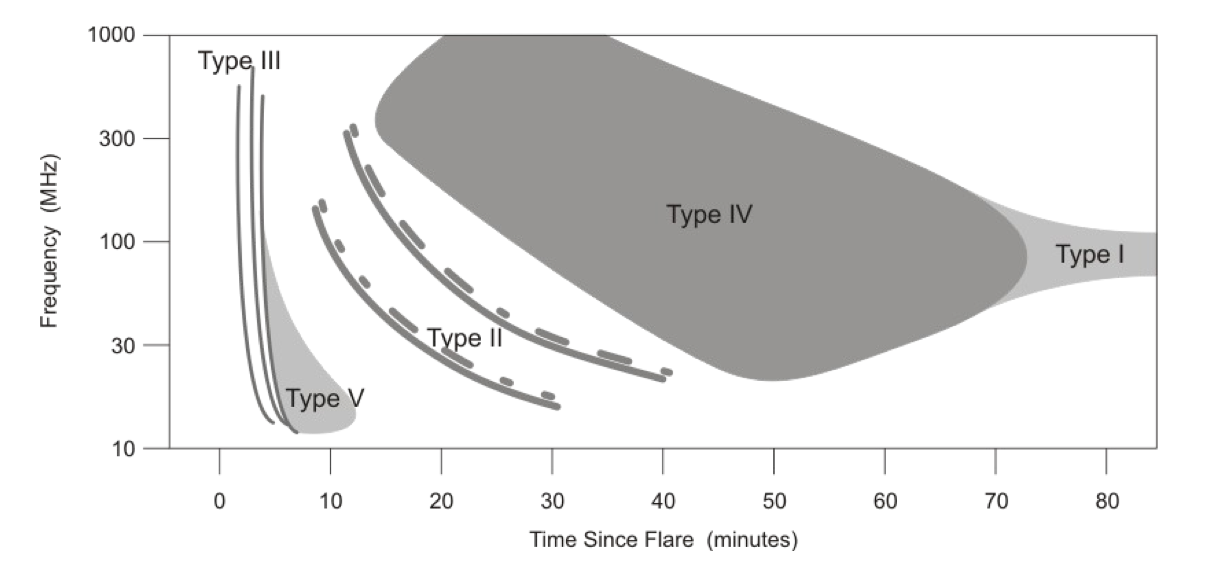
\includegraphics[scale=0.35, trim=2cm 0cm 0cm 2cm]{radiobursts.png}
\caption[Solar radio burst morphologies]{The characteristic shapes of various solar radio bursts seen in dynamic spectra. Type II radio burst are a signature of shock transit from high number density into low number density, as indicated by their drift from high to low frequency. The presence of two distinct bands is indicative of radio emission at the plasma frequency (fundamental) and its second harmonic. These two bands may also be further split themselves, a feature known as band-splitting.}
\label{fig:radiobursts}
\end{center}
\end{figure}

Generally, the frequency drift of the radio burst depends on the velocity of the exciter and the density variation in the corona. It is possible to estimate the speed of the exciter from a set of frequency time values $(f_i, t_i)$. Such as set of values are a direct diagnostic of the number density of the environment of emission versus time e.g., using $f \approx 9000\sqrt{n_e}$, frequency versus time gives number density versus time, $(f_i, t_i) \rightarrow (n_i,t_i)$.
Now, in general the number density of the corona is inversely proportional to height, varying according to some exponential decrease. A very simple model is the hydrostatic case $n(r) = n_0\mathrm{exp}(-r/H)$
\begin{figure}[t!]
%\begin{center}
\begin{minipage}[]{0.5\linewidth}
\centering
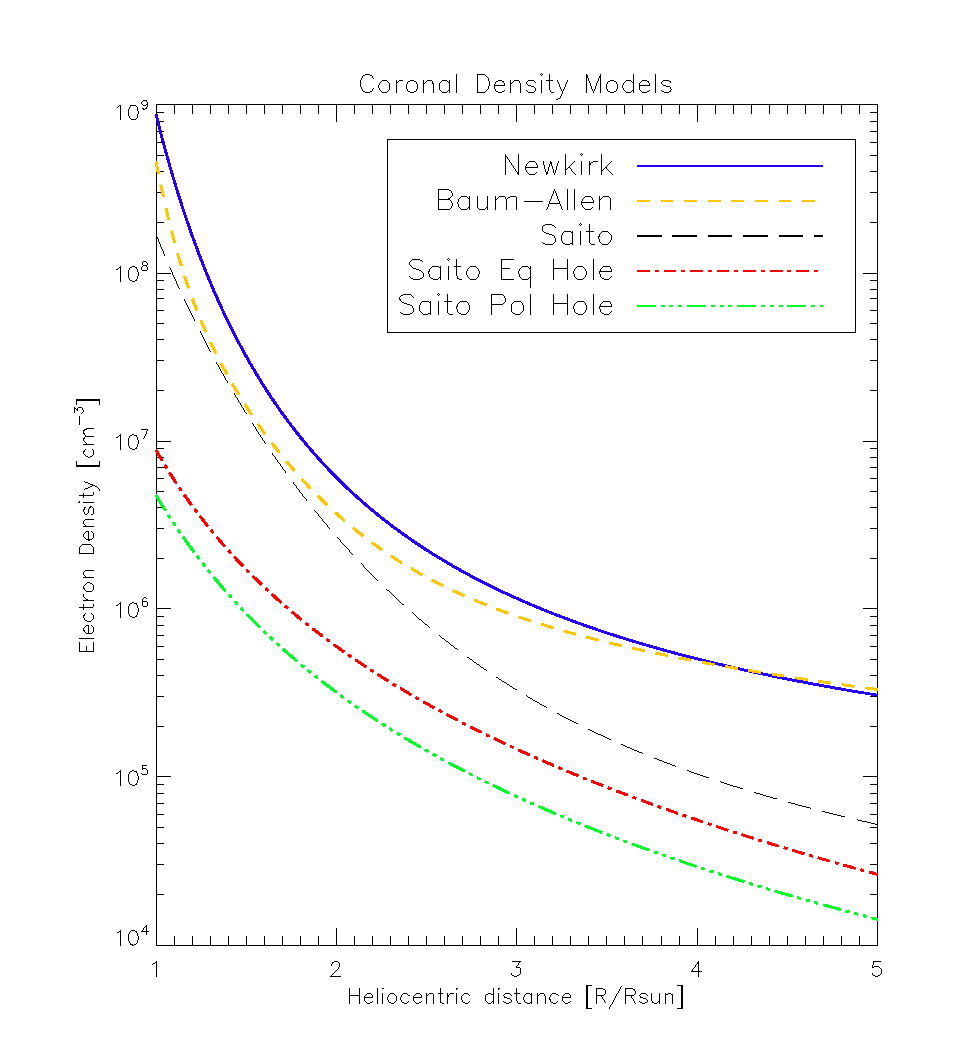
\includegraphics[trim= 2cm 0.0cm 0.0cm 2.0cm, scale=0.4]{density_models.pdf}
\end{minipage}
\hspace{0.1cm}
\begin{minipage}[]{0.3\linewidth}
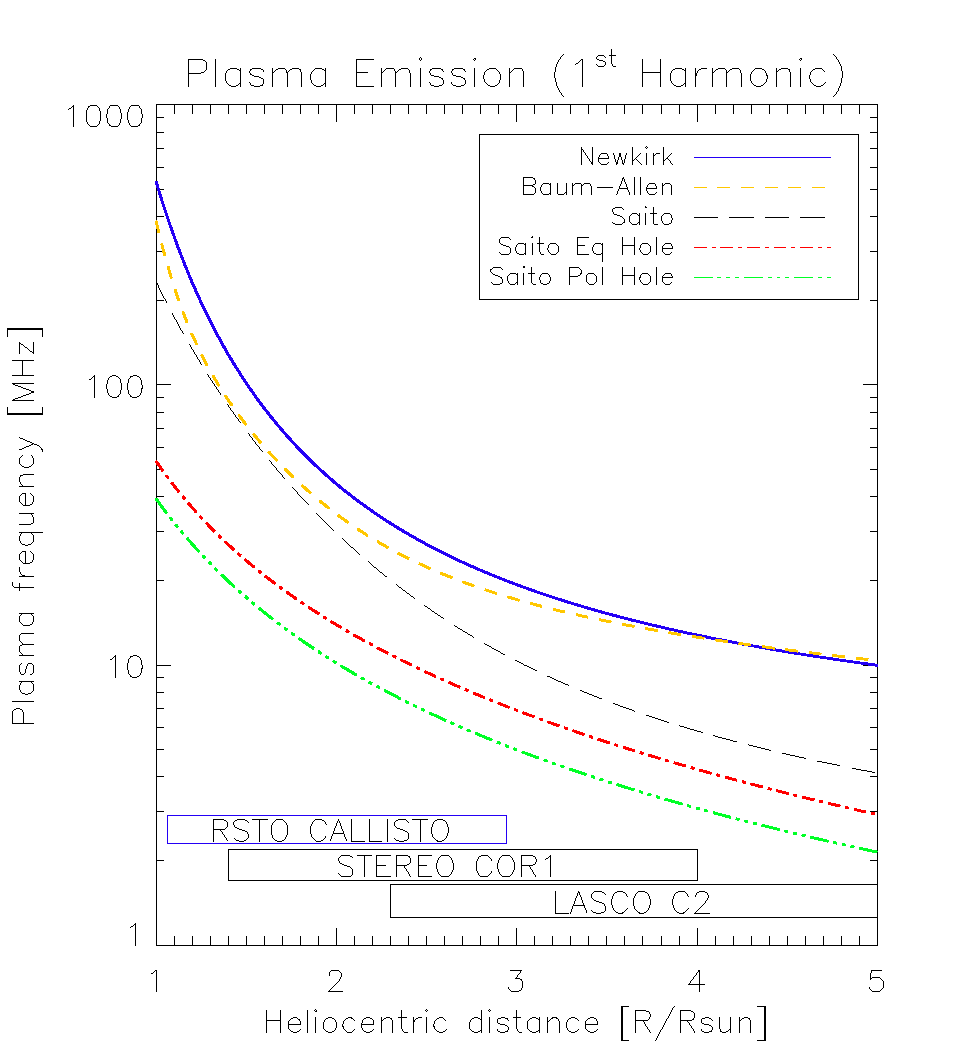
\includegraphics[scale=0.4, trim= 0cm 0.0cm 0.0cm 2.0cm]{1st_harmonic.pdf}
\end{minipage}
\caption[Various models for electron number density in the corona]{(Left)\,Electron number density as a function of height as defined by each of the models listed. The Newkirk, Baumbach Allen, and Saito models each describe an equatorial quiet corona electron density profile. The Saito Eq Hole and Pol Hol describe equatorial and polar hole profiles, respectively. These models are generally used to specify the height of a radio burst in the corona, and the choice of model is often arbitrary. (Right) The first harmonic of the plasma frequency as a function of height defined by the models.}% Added text here to elaborate differences between models
\label{fig:frequency_model}
\end{figure}
where $r$ is distance from sun center, and $H$ is the scale height given by $H = kT/mg$, where $k$ is Boltzman's constant, $T$ is the coronal temperature, $m$ is proton mass and $g$ is gravity. Generally using this $n(r)$, the set of values $(n_i,t_i)$ can be converted to as set of $(r_i,t_i)$
\begin{equation}
(f_i, t_i) \rightarrow (n_i,t_i) \rightarrow n(r) \rightarrow (r_i,t_i).
\end{equation}
Hence, by some appropriate choice of coronal density model $n(r)$, a set of frequency and time values may be converted to a set of height vs time values, from which the velocity may be derived.
%The derived shock velocity firstly assumes purely radial propagation of the shock, which is most likely not the case, and more importantly the method relies heavily on the choice of density model $n(r)$. 
Common practice is to use an $n(r)$ that is derived semi-empirically. For example, there exists a set of models that describe the density fall off with height of the equatorial quiet corona, coronal holes, and active regions \citet{allen1947, newkirk1961, saito1977}, shown in Figure~\ref{fig:frequency_model}. The choice of model affects both the resulting height of the radio emission and the derived speed. A much better diagnostic of radio bursts would be to use actual density measurements of the corona in places of these models, but this is generally not usual practice.

%In Figure 3.5 (left), there is a noticeable difference in both the range of densities and rate of decrease between each of these models. The choice of model to be used in the analysis of type II events is usually determined by the conditions that the shock is assumed to be propagating in. For example there could be propagation in an equatorial or polar coronal hole, through a quiet coronal background, or near an active region or streamer; the electron density is also known to vary with the cycle \citep{lamy2002}. 

%The choice of model affects both the resulting height of the radio emission and the derived speed. Also, even if the shock is known to be propagating in quiet coronal densities there is still a choice between a variety of models, such as the Saito, Newkirk and Baumbach-Allen models, each of which describe quiet equatorial corona. There is a noticeable difference between these models and the choice of one or the other, which is often arbitrary, will effect the resulting shock properties. Ultimately, the analysis of radio bursts are very heavily dependent on the coronal density model that is used, and there is no reason to favor one model over another.














% --------------------------------------------------------------
%:                  BACK MATTER: appendices, refs,..
% --------------------------------------------------------------
\appendix

%!TEX root = ../thesis.tex
%Adding the above line, with the name of your base .tex file (in this case "thesis.tex") will allow you to compile the whole thesis even when working inside one of the chapter tex files

\chapter{A Nice Appendix}
\label{app:1}

If we assume the herringbones are due to the shock drift acceleration process then the velocity upon a reflection from the shock is
\begin{equation}
v_{r,||} = 2v_{shock}\mathrm{sec}\,\theta_{Bn} - v_{i,||}
\end{equation}
where $v_{r,||}$ is the reflected parallel velocity of the particle, $v_{i,||}$ is the incident parallel velocity of the paticle, $v_{shock}$ is the shock velocity, and $\theta$ is the angle between upstream $B-$field and shock normal $n$. Taking the shock speed to be the speed of the 150\,MHz radio source, $550\times10^3$\,m\,s$^{-1}$, and $v_{i,||}$ to be the thermal speed of an electron 
\begin{equation} 
v_{thermal} = \sqrt{ \frac{3k_bT}{m_e} }
\end{equation}
At $1\times10^{6}$\,K, $v_{thermal} = v_{i,||} = 6.7\times10^6$\,m\,s$^{-1}$. Now, the herringbone electron speed 0.15\,c, this is the reflected speed $v_{r,||}$ in equation A1. Rearranging A1 we get
\begin{equation}
\theta_{Bn} = \mathrm{sec}^{-1}\bigg( \frac{1}{2}\frac{v_{r,||} +  v_{i,||} }{v_{shock}}\bigg)
\end{equation}
Substituting the above values we get $\theta_{Bn}=88^{\circ}$. Independent verification of a quasi-perpendicular shock orientation!



\section{Radio burst intensity}


\begin{equation}
\Phi_F \approx 72\sqrt{3}   \frac{\gamma_{L^{'}}}{\gamma_S}   \frac{v_e^3}{c^3}   \frac{v_b}{\Delta v_b}   \frac{e^{-u_c^2}}{u_c\sqrt{\pi}}  \zeta_F
\end{equation}
\begin{equation}
\Phi_H \approx \frac{18\sqrt{3}}{5\gamma_t}   \sqrt{\frac{m_i}{\gamma_t m_e}}  \frac{v_e^3 v_b^3}{c^5} \frac{v_b}{\Delta v_b}\zeta_H
\end{equation}
the expression involving $u_c$ represent an \textquoteleft escape factor' for the fundamental taking into account absorption and scattering of the radiation. $ \frac{\gamma_{L^{'}}}{\gamma_S} $ is the ratio of the damping rates of the product waves out of processes in equations~\ref{eqn:harm} and \ref{eqn:fund}. The $\zeta$ terms are the fractions of Langmuir waves that are kinematically able to contribute to the fundamental or harmonic emission, given by

\begin{equation}
\zeta_F  \approx \mathrm{exp} \bigg[  -\frac{4\gamma_t m_e}{45 m_i}    \bigg(\frac{v_b}{\Delta v_b}\bigg)^2   \bigg(  \frac{3}{2}  \sqrt{\frac{m_i}{\gamma_t m_e}} - \frac{v_b}{v_e}  \bigg)^2    \bigg]
\end{equation}

\begin{equation}
\zeta_H \approx \frac{c}{2v_b} \sqrt{\frac{\pi}{6}} \frac{\beta \Delta v_b}{v_b}
\Bigg[  \mathrm{erf}\Bigg(     \frac{ \frac{v_e\sqrt{3}}{c}  + \frac{2}{3} \sqrt{\frac{\gamma_t m_e}{m_i}}  }  {\frac{v_e}{v_b} \frac{\beta \Delta v_b}{v_b} \sqrt{2} }   \Bigg)     +   \mathrm{erf}\Bigg(     \frac{ \frac{v_e\sqrt{3}}{c}  - \frac{2}{3} \sqrt{\frac{\gamma_t m_e}{m_i}}  }  {\frac{v_e}{v_b} \frac{\beta \Delta v_b}{v_b} \sqrt{2} }   \Bigg)   \Bigg]
\end{equation}
where erf is the error function. 


\section{Band-splitting}
Using a ploytropic index of $\gamma=5/3$ (monatomic) means the shock compression can be no more than a factor of 4. Another extremely important fact arising from this is that magnetic compression can also be no greater than 4 i.e., from equation 4(b) $B_{2}/B_{1}=\chi$. $\chi<4$ has consequences for the shock drift acceleration mechanism and provides an upper limit to the particle energy gain

may also provide an upper limit to the level of band splitting in type II radio bursts (since this effect is thought to be related to the emission induced up/downstream of the shock). Although the maximum compression ration of 4 was derived from the roots of the quadratic for $\chi$ for the perpendicular shock, a similar analysis for the much more general oblique shock also leads to the same result. The density compression and tangential magnetic compression can be no more than a factor of $(\gamma+1)/(\gamma-1)$ for any MHD shock. 

%In either the perpendicular case or the general 2D oblique case a polynomial expression for the compression ratio (such as (6)) may be derived. The general oblique shock case requires extra terms in the polynomial such as $M_{A},\beta,\gamma,\theta_{Bn},\theta_{vn}$ ($\theta_{Bn}$ is the angle between shock normal and magnetic field, and $\theta_vn$ is the angle between shock normal and plasma flow). 
Polynomials such as (6) are extremely useful, and can lead to simple expressions for the Alfv\'{e}nic-Mach number in terms of $\chi$, in this case
\begin{equation}
M_{A}=\sqrt{\frac{\chi(\chi+5+5\beta)}{2(4-\chi)}} 
\end{equation}
for a perpendicular shock. If the shock speed and compression ratio are known, this equation provides a means of measuring the Alfv\'{e}n speed in the shock medium. 

This technique is exploited in the analysis of type II radio bursts. As the shock propagates into the corona it emits EM radiation at the local plasma frequency (1) (see section 4), and since the density drops as the shock travels into the heliosphere, so too does the frequency of emission. From frequency drift rate an estimate of shock speed is possible. If band splitting of the emission is present this is interpreted as emission from upstream and downstream of the shock, which provides a diagnostic of upstream/downstream densities via (1) and hence an estimate of $\chi$ \citep{vrsnak2002}. However, use of (8) in calculating Mach number and Alfv\'{e}n speed in the corona has some clear shortcomings such that it clearly ignores any dependency of the angle between magnetic field, velocity vector and shock normal i.e., (8) only applies to a purely perpendicular shock.

The general oblique shock case requires extra terms in the polynomial such as $\theta_{Bn}$ and $\theta_{vn}$ ($\theta_{Bn}$ is the angle between shock normal and magnetic field, and $\theta_{vn}$ is the angle between shock normal and plasma flow). For the oblique case the polynomial becomes
\begin{equation}
(A^2-\chi)^2\bigg[A^2 - \frac{2\chi S^2}{\chi+1-\gamma(\chi-1)}\bigg]\\
-\chi k^2A^2\bigg[\frac{2\chi - \gamma(\chi-1)}{\chi+1- \gamma(\chi-1)}A^2 -\chi\bigg]=0
\end{equation}
where $A=\frac{M_A\mathrm{cos}\theta_{vn}}{cos(\theta_{Bv}-\theta_{bn})}$,  $S=\frac{c_s}{v_A}$, $k=\mathrm{tan}(\theta_{vn}-\theta_{Bv})$ \footnote{$\theta_{Bv}$ is angle between magnetic field and velocity vector, it has a simple relationship with $\theta_{Bn}$} 
\citep{kabin2001}. Equation (6) is a quadratic of variable $\chi$, the more general equation (9) is a cubic equation for $\chi$, the roots of which give the compression for the oblique case. Since it is a function of $M_A$, $\theta_{vn}$, and $\theta_{bv}$, $\chi$ may have a range of values depending not only on Mach number but also shock orientation. Figure 2 illustrates the broad range in compressions of 0$<\chi<$3.5 across the shock depending on both flow and magnetic field orientation with respect to the shock normal, and in this case $M_A=2.5$. 
%\begin{figure}[h!]
%\includegraphics[scale=0.5, angle=270,trim =  3cm 0cm 4cm 0cm]{data/vary_thetaVn_thetaBn_mach2_5.pdf}
%\caption{Image and surface plot of compression ratio (from the solutions of (9)) as a function of $\theta_{vn}$ and $\theta_{Bn}$, with an Alfv\'{e}n Mach number of 2.5. The range of compressions is from 0 to 3.5 depending on the orientation of the magnetic field and velocity vectors with respect to the shock normal. Any discontinuities or sharp jumps are an indication of where the solutions to (9) are multi-valued.}
%\label{fig:vary_thetaVn_thetaBn_mach2_5}
%\end{figure}
This is a very general case, however, permitting any angle of orentation of $B$ and $v$. Since type II bursts are thought to be from shocks that are quasi perpendicular, this places restriction on the values for $\theta_{vn}$, and $\theta_{Bn}$, especially when the flow is considered to be head-on i.e. $\theta_{vn}=0^{\circ}$. Therefore in the quasi-perpendicular case their is a tighter constraint on the amount of compression across the shock. Further constraining the Mach number to a limited range of values puts quite a limiting range on the compression ratio, and hence a limiting range of band splitting of type II radio bursts since $f_{plasma}\approx9000\sqrt{n_e}$, hence
\begin{equation}
\delta_{bs} \equiv \frac{f_{upper}}{f_{lower}} \approx \sqrt{ \frac{ n_{e,d} }{ n_{e,u} } }=\sqrt{\chi}
\end{equation}
where $n_{e,d}$ and $n_{e,u}$ are downstream and upstream plasma number densities, and $\delta_{bs}$ is the ratio of upper to lower band frequencies, $f_{upper}$ and $f_{lower}$ respectively, in a split radio burst. Figure 3 shows the expected range in band splitting ($\delta_{bs}=\sqrt{\chi}$) for a type II given a range in Alfv\'{e}n Mach numbers $1<M_A< 4$, and quasi-perpendicular magnetic field orientations $45^{\circ}<\theta_{Bn}<90^{\circ}$. 
\begin{figure}[h!]
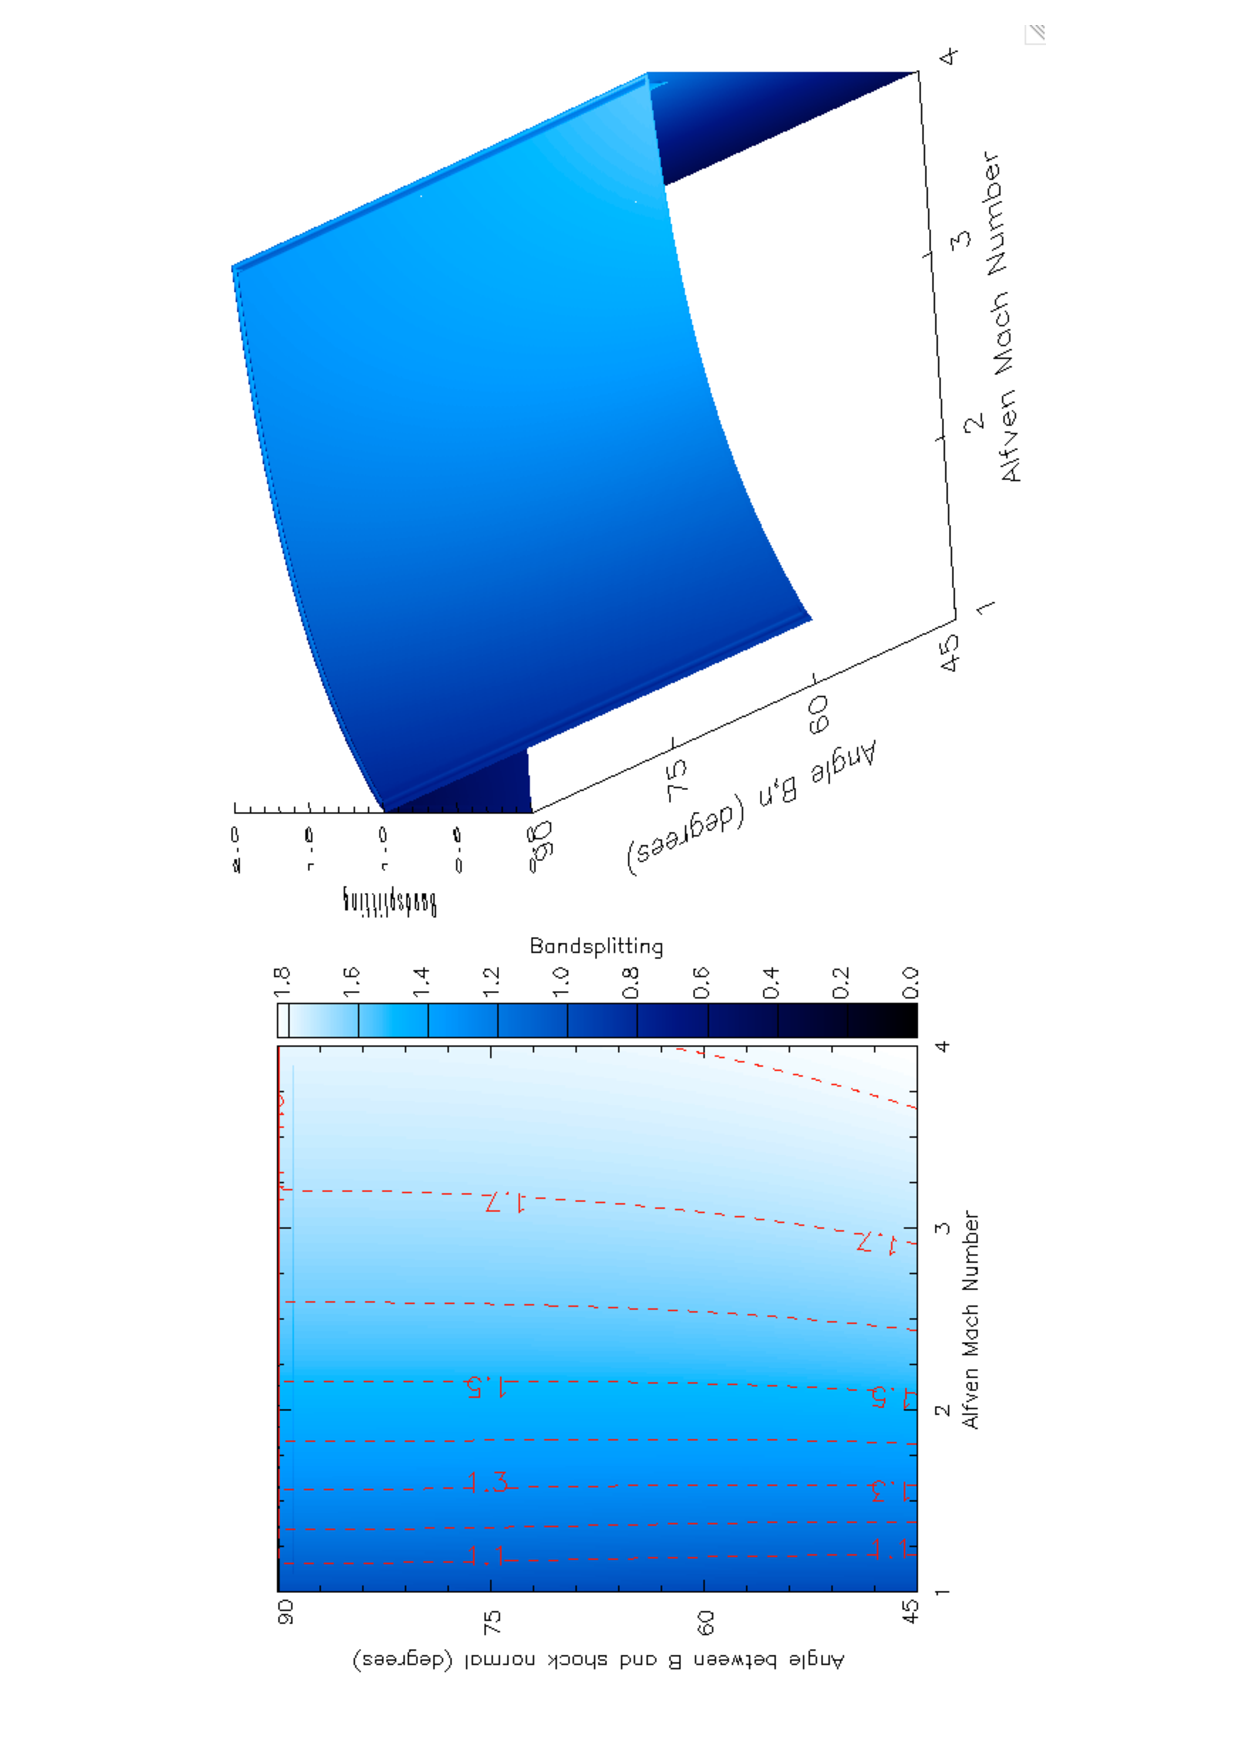
\includegraphics[scale=0.5, angle=270,trim =  3cm 0cm 4cm 0cm]{images/MHD_vary_mach&thetaBn.pdf}
\caption{Predicted band splitting ratio $\delta_{bs}$ as a function of Mach number and magnetic field orientation with respect to shock normal. Flow is anti-parallel to shock normal (head-on). Both image and surface are shown, left and right respectively. On the left, the red contours show specific values of of band-splitting. Note that for small mach numbers the level of band splitting is independent of magnetic field orientation. It is only at Mach numbers greater than $\sim$2.1 that the B-field orientation becomes important.}
\label{fig:MHD_vary_mach&thetaBn}
\end{figure}
This analysis shows that for a quasi-perpendicular shock the theoretically predicted range in type II band-spliting is $1<\delta_{bs}<1.8$. Such an upper limit to the level of band-splitting seems excessive and is probably due to a large upper limit to the Mach number being used to calculate the compression ratio. This is especially relevant in the low corona where Alfv\'{e}n speed can be quite large, making it difficult for a CME or blast wave to drive a shock at $M_A=4$. Also, given a typical band-splitting ratio of $\delta_{bs}=1.21\pm0.7$ at metric wavelengths \citep{vrsnak2004}, this would indicate typical Alfv\'{e}n-Mach number of $\sim\,1.5$ in the low corona. This seems reasonable, however Mach numbers of $\sim$3 are possible, and figure 3 would suggest a possible band-split ratio of $\delta_{bs}\sim1.7$ for such a Mach number. Such a level of band-splitting seems very unlikely, suggesting a quasi-perpendicular shock with a head on flow is a limiting case. More likely is a quasi-perpendicular shock with a flow orientation $\theta_{vn}\neq0$. For example if $\theta_{Bn}=90^{\circ}$ and $\theta_{vn}=45^{\circ}$ then band splitting can be $\delta_{bs}\sim\,1.5$ for $M_A$=3, which is under the upper limit of observed type II band-split ratios of $\sim\,1.58$. Allowing $\theta_{vn}\neq0$ can allow larger, more realistic Mach numbers to produce smaller and more realistic bandsplitting.


It is clear that the distribution in the level of band splitting in type II radio bursts depends not only on Mach number but the relative orientations of flow and magnetic field with respect to shock normal. A statistical analysis could possibly give an observationally predicted distribution in $\theta_{Bn}$ (provided $M_A$ is known) that would confirm the quasi-perpendicularlity of type II-generating shocks.




%: ----------------------- bibliography ------------------------

\begin{footnotesize} 
\bibliographystyle{Latex/Classes/jmb}
\renewcommand{\bibname}{References} 
\bibliography{mybib} 
\end{footnotesize}


\end{document}
